% Electronic Supplementary Material (ESM) of the VLDB Journal submission of
% PhaseFormer. It collects the supplementary material of the ICLR 2026
% conference version (formerly Appendix A of the main PDF), moved out of the
% main manuscript to meet the 25-page limit. Build like the main PDF:
%   latexmk -pdf supplementary.tex
\RequirePackage{fix-cm}
% VLDBJ requires numbered citations in square brackets.
\PassOptionsToPackage{numbers,sort&compress}{natbib}
\documentclass[twocolumn,natbib]{svjour3}
\bibpunct{[}{]}{,}{n}{}{,}
% The supplement writes ``Model~\citeyearpar{key}''; render it as a numbered citation.
\renewcommand{\citeyearpar}{\unskip~\citep}
\smartqed

\usepackage[T1]{fontenc}
\usepackage{times}
\usepackage[protrusion=true,expansion=true]{microtype}
\usepackage{amsmath,amssymb}
\usepackage{graphicx}
\usepackage{multirow}
\usepackage{booktabs}
\usepackage{xspace}
\usepackage{enumitem}
\usepackage{xcolor}
\usepackage{subcaption}
\usepackage{url}
\usepackage[hidelinks]{hyperref}
\usepackage{xurl}

% Optional math commands from https://github.com/goodfeli/dlbook_notation.
%%%%% NEW MATH DEFINITIONS %%%%%

\usepackage{amsmath,amsfonts,bm}

% Mark sections of captions for referring to divisions of figures
\newcommand{\figleft}{{\em (Left)}}
\newcommand{\figcenter}{{\em (Center)}}
\newcommand{\figright}{{\em (Right)}}
\newcommand{\figtop}{{\em (Top)}}
\newcommand{\figbottom}{{\em (Bottom)}}
\newcommand{\captiona}{{\em (a)}}
\newcommand{\captionb}{{\em (b)}}
\newcommand{\captionc}{{\em (c)}}
\newcommand{\captiond}{{\em (d)}}

% Highlight a newly defined term
\newcommand{\newterm}[1]{{\bf #1}}


% Figure reference, lower-case.
\def\figref#1{figure~\ref{#1}}
% Figure reference, capital. For start of sentence
\def\Figref#1{Figure~\ref{#1}}
\def\twofigref#1#2{figures \ref{#1} and \ref{#2}}
\def\quadfigref#1#2#3#4{figures \ref{#1}, \ref{#2}, \ref{#3} and \ref{#4}}
% Section reference, lower-case.
\def\secref#1{section~\ref{#1}}
% Section reference, capital.
\def\Secref#1{Section~\ref{#1}}
% Reference to two sections.
\def\twosecrefs#1#2{sections \ref{#1} and \ref{#2}}
% Reference to three sections.
\def\secrefs#1#2#3{sections \ref{#1}, \ref{#2} and \ref{#3}}
% Reference to an equation, lower-case.
\def\eqref#1{equation~\ref{#1}}
% Reference to an equation, upper case
\def\Eqref#1{Equation~\ref{#1}}
% A raw reference to an equation---avoid using if possible
\def\plaineqref#1{\ref{#1}}
% Reference to a chapter, lower-case.
\def\chapref#1{chapter~\ref{#1}}
% Reference to an equation, upper case.
\def\Chapref#1{Chapter~\ref{#1}}
% Reference to a range of chapters
\def\rangechapref#1#2{chapters\ref{#1}--\ref{#2}}
% Reference to an algorithm, lower-case.
\def\algref#1{algorithm~\ref{#1}}
% Reference to an algorithm, upper case.
\def\Algref#1{Algorithm~\ref{#1}}
\def\twoalgref#1#2{algorithms \ref{#1} and \ref{#2}}
\def\Twoalgref#1#2{Algorithms \ref{#1} and \ref{#2}}
% Reference to a part, lower case
\def\partref#1{part~\ref{#1}}
% Reference to a part, upper case
\def\Partref#1{Part~\ref{#1}}
\def\twopartref#1#2{parts \ref{#1} and \ref{#2}}

\def\ceil#1{\lceil #1 \rceil}
\def\floor#1{\lfloor #1 \rfloor}
\def\1{\bm{1}}
\newcommand{\train}{\mathcal{D}}
\newcommand{\valid}{\mathcal{D_{\mathrm{valid}}}}
\newcommand{\test}{\mathcal{D_{\mathrm{test}}}}

\def\eps{{\epsilon}}


% Random variables
\def\reta{{\textnormal{$\eta$}}}
\def\ra{{\textnormal{a}}}
\def\rb{{\textnormal{b}}}
\def\rc{{\textnormal{c}}}
\def\rd{{\textnormal{d}}}
\def\re{{\textnormal{e}}}
\def\rf{{\textnormal{f}}}
\def\rg{{\textnormal{g}}}
\def\rh{{\textnormal{h}}}
\def\ri{{\textnormal{i}}}
\def\rj{{\textnormal{j}}}
\def\rk{{\textnormal{k}}}
\def\rl{{\textnormal{l}}}
% rm is already a command, just don't name any random variables m
\def\rn{{\textnormal{n}}}
\def\ro{{\textnormal{o}}}
\def\rp{{\textnormal{p}}}
\def\rq{{\textnormal{q}}}
\def\rr{{\textnormal{r}}}
\def\rs{{\textnormal{s}}}
\def\rt{{\textnormal{t}}}
\def\ru{{\textnormal{u}}}
\def\rv{{\textnormal{v}}}
\def\rw{{\textnormal{w}}}
\def\rx{{\textnormal{x}}}
\def\ry{{\textnormal{y}}}
\def\rz{{\textnormal{z}}}

% Random vectors
\def\rvepsilon{{\mathbf{\epsilon}}}
\def\rvtheta{{\mathbf{\theta}}}
\def\rva{{\mathbf{a}}}
\def\rvb{{\mathbf{b}}}
\def\rvc{{\mathbf{c}}}
\def\rvd{{\mathbf{d}}}
\def\rve{{\mathbf{e}}}
\def\rvf{{\mathbf{f}}}
\def\rvg{{\mathbf{g}}}
\def\rvh{{\mathbf{h}}}
\def\rvu{{\mathbf{i}}}
\def\rvj{{\mathbf{j}}}
\def\rvk{{\mathbf{k}}}
\def\rvl{{\mathbf{l}}}
\def\rvm{{\mathbf{m}}}
\def\rvn{{\mathbf{n}}}
\def\rvo{{\mathbf{o}}}
\def\rvp{{\mathbf{p}}}
\def\rvq{{\mathbf{q}}}
\def\rvr{{\mathbf{r}}}
\def\rvs{{\mathbf{s}}}
\def\rvt{{\mathbf{t}}}
\def\rvu{{\mathbf{u}}}
\def\rvv{{\mathbf{v}}}
\def\rvw{{\mathbf{w}}}
\def\rvx{{\mathbf{x}}}
\def\rvy{{\mathbf{y}}}
\def\rvz{{\mathbf{z}}}

% Elements of random vectors
\def\erva{{\textnormal{a}}}
\def\ervb{{\textnormal{b}}}
\def\ervc{{\textnormal{c}}}
\def\ervd{{\textnormal{d}}}
\def\erve{{\textnormal{e}}}
\def\ervf{{\textnormal{f}}}
\def\ervg{{\textnormal{g}}}
\def\ervh{{\textnormal{h}}}
\def\ervi{{\textnormal{i}}}
\def\ervj{{\textnormal{j}}}
\def\ervk{{\textnormal{k}}}
\def\ervl{{\textnormal{l}}}
\def\ervm{{\textnormal{m}}}
\def\ervn{{\textnormal{n}}}
\def\ervo{{\textnormal{o}}}
\def\ervp{{\textnormal{p}}}
\def\ervq{{\textnormal{q}}}
\def\ervr{{\textnormal{r}}}
\def\ervs{{\textnormal{s}}}
\def\ervt{{\textnormal{t}}}
\def\ervu{{\textnormal{u}}}
\def\ervv{{\textnormal{v}}}
\def\ervw{{\textnormal{w}}}
\def\ervx{{\textnormal{x}}}
\def\ervy{{\textnormal{y}}}
\def\ervz{{\textnormal{z}}}

% Random matrices
\def\rmA{{\mathbf{A}}}
\def\rmB{{\mathbf{B}}}
\def\rmC{{\mathbf{C}}}
\def\rmD{{\mathbf{D}}}
\def\rmE{{\mathbf{E}}}
\def\rmF{{\mathbf{F}}}
\def\rmG{{\mathbf{G}}}
\def\rmH{{\mathbf{H}}}
\def\rmI{{\mathbf{I}}}
\def\rmJ{{\mathbf{J}}}
\def\rmK{{\mathbf{K}}}
\def\rmL{{\mathbf{L}}}
\def\rmM{{\mathbf{M}}}
\def\rmN{{\mathbf{N}}}
\def\rmO{{\mathbf{O}}}
\def\rmP{{\mathbf{P}}}
\def\rmQ{{\mathbf{Q}}}
\def\rmR{{\mathbf{R}}}
\def\rmS{{\mathbf{S}}}
\def\rmT{{\mathbf{T}}}
\def\rmU{{\mathbf{U}}}
\def\rmV{{\mathbf{V}}}
\def\rmW{{\mathbf{W}}}
\def\rmX{{\mathbf{X}}}
\def\rmY{{\mathbf{Y}}}
\def\rmZ{{\mathbf{Z}}}

% Elements of random matrices
\def\ermA{{\textnormal{A}}}
\def\ermB{{\textnormal{B}}}
\def\ermC{{\textnormal{C}}}
\def\ermD{{\textnormal{D}}}
\def\ermE{{\textnormal{E}}}
\def\ermF{{\textnormal{F}}}
\def\ermG{{\textnormal{G}}}
\def\ermH{{\textnormal{H}}}
\def\ermI{{\textnormal{I}}}
\def\ermJ{{\textnormal{J}}}
\def\ermK{{\textnormal{K}}}
\def\ermL{{\textnormal{L}}}
\def\ermM{{\textnormal{M}}}
\def\ermN{{\textnormal{N}}}
\def\ermO{{\textnormal{O}}}
\def\ermP{{\textnormal{P}}}
\def\ermQ{{\textnormal{Q}}}
\def\ermR{{\textnormal{R}}}
\def\ermS{{\textnormal{S}}}
\def\ermT{{\textnormal{T}}}
\def\ermU{{\textnormal{U}}}
\def\ermV{{\textnormal{V}}}
\def\ermW{{\textnormal{W}}}
\def\ermX{{\textnormal{X}}}
\def\ermY{{\textnormal{Y}}}
\def\ermZ{{\textnormal{Z}}}

% Vectors
\def\vzero{{\bm{0}}}
\def\vone{{\bm{1}}}
\def\vmu{{\bm{\mu}}}
\def\vtheta{{\bm{\theta}}}
\def\va{{\bm{a}}}
\def\vb{{\bm{b}}}
\def\vc{{\bm{c}}}
\def\vd{{\bm{d}}}
\def\ve{{\bm{e}}}
\def\vf{{\bm{f}}}
\def\vg{{\bm{g}}}
\def\vh{{\bm{h}}}
\def\vi{{\bm{i}}}
\def\vj{{\bm{j}}}
\def\vk{{\bm{k}}}
\def\vl{{\bm{l}}}
\def\vm{{\bm{m}}}
\def\vn{{\bm{n}}}
\def\vo{{\bm{o}}}
\def\vp{{\bm{p}}}
\def\vq{{\bm{q}}}
\def\vr{{\bm{r}}}
\def\vs{{\bm{s}}}
\def\vt{{\bm{t}}}
\def\vu{{\bm{u}}}
\def\vv{{\bm{v}}}
\def\vw{{\bm{w}}}
\def\vx{{\bm{x}}}
\def\vy{{\bm{y}}}
\def\vz{{\bm{z}}}

% Elements of vectors
\def\evalpha{{\alpha}}
\def\evbeta{{\beta}}
\def\evepsilon{{\epsilon}}
\def\evlambda{{\lambda}}
\def\evomega{{\omega}}
\def\evmu{{\mu}}
\def\evpsi{{\psi}}
\def\evsigma{{\sigma}}
\def\evtheta{{\theta}}
\def\eva{{a}}
\def\evb{{b}}
\def\evc{{c}}
\def\evd{{d}}
\def\eve{{e}}
\def\evf{{f}}
\def\evg{{g}}
\def\evh{{h}}
\def\evi{{i}}
\def\evj{{j}}
\def\evk{{k}}
\def\evl{{l}}
\def\evm{{m}}
\def\evn{{n}}
\def\evo{{o}}
\def\evp{{p}}
\def\evq{{q}}
\def\evr{{r}}
\def\evs{{s}}
\def\evt{{t}}
\def\evu{{u}}
\def\evv{{v}}
\def\evw{{w}}
\def\evx{{x}}
\def\evy{{y}}
\def\evz{{z}}

% Matrix
\def\mA{{\bm{A}}}
\def\mB{{\bm{B}}}
\def\mC{{\bm{C}}}
\def\mD{{\bm{D}}}
\def\mE{{\bm{E}}}
\def\mF{{\bm{F}}}
\def\mG{{\bm{G}}}
\def\mH{{\bm{H}}}
\def\mI{{\bm{I}}}
\def\mJ{{\bm{J}}}
\def\mK{{\bm{K}}}
\def\mL{{\bm{L}}}
\def\mM{{\bm{M}}}
\def\mN{{\bm{N}}}
\def\mO{{\bm{O}}}
\def\mP{{\bm{P}}}
\def\mQ{{\bm{Q}}}
\def\mR{{\bm{R}}}
\def\mS{{\bm{S}}}
\def\mT{{\bm{T}}}
\def\mU{{\bm{U}}}
\def\mV{{\bm{V}}}
\def\mW{{\bm{W}}}
\def\mX{{\bm{X}}}
\def\mY{{\bm{Y}}}
\def\mZ{{\bm{Z}}}
\def\mBeta{{\bm{\beta}}}
\def\mPhi{{\bm{\Phi}}}
\def\mLambda{{\bm{\Lambda}}}
\def\mSigma{{\bm{\Sigma}}}

% Tensor
\DeclareMathAlphabet{\mathsfit}{\encodingdefault}{\sfdefault}{m}{sl}
\SetMathAlphabet{\mathsfit}{bold}{\encodingdefault}{\sfdefault}{bx}{n}
\providecommand{\tens}[1]{\bm{\mathsfit{#1}}}
\def\tA{{\tens{A}}}
\def\tB{{\tens{B}}}
\def\tC{{\tens{C}}}
\def\tD{{\tens{D}}}
\def\tE{{\tens{E}}}
\def\tF{{\tens{F}}}
\def\tG{{\tens{G}}}
\def\tH{{\tens{H}}}
\def\tI{{\tens{I}}}
\def\tJ{{\tens{J}}}
\def\tK{{\tens{K}}}
\def\tL{{\tens{L}}}
\def\tM{{\tens{M}}}
\def\tN{{\tens{N}}}
\def\tO{{\tens{O}}}
\def\tP{{\tens{P}}}
\def\tQ{{\tens{Q}}}
\def\tR{{\tens{R}}}
\def\tS{{\tens{S}}}
\def\tT{{\tens{T}}}
\def\tU{{\tens{U}}}
\def\tV{{\tens{V}}}
\def\tW{{\tens{W}}}
\def\tX{{\tens{X}}}
\def\tY{{\tens{Y}}}
\def\tZ{{\tens{Z}}}


% Graph
\def\gA{{\mathcal{A}}}
\def\gB{{\mathcal{B}}}
\def\gC{{\mathcal{C}}}
\def\gD{{\mathcal{D}}}
\def\gE{{\mathcal{E}}}
\def\gF{{\mathcal{F}}}
\def\gG{{\mathcal{G}}}
\def\gH{{\mathcal{H}}}
\def\gI{{\mathcal{I}}}
\def\gJ{{\mathcal{J}}}
\def\gK{{\mathcal{K}}}
\def\gL{{\mathcal{L}}}
\def\gM{{\mathcal{M}}}
\def\gN{{\mathcal{N}}}
\def\gO{{\mathcal{O}}}
\def\gP{{\mathcal{P}}}
\def\gQ{{\mathcal{Q}}}
\def\gR{{\mathcal{R}}}
\def\gS{{\mathcal{S}}}
\def\gT{{\mathcal{T}}}
\def\gU{{\mathcal{U}}}
\def\gV{{\mathcal{V}}}
\def\gW{{\mathcal{W}}}
\def\gX{{\mathcal{X}}}
\def\gY{{\mathcal{Y}}}
\def\gZ{{\mathcal{Z}}}

% Sets
\def\sA{{\mathbb{A}}}
\def\sB{{\mathbb{B}}}
\def\sC{{\mathbb{C}}}
\def\sD{{\mathbb{D}}}
% Don't use a set called E, because this would be the same as our symbol
% for expectation.
\def\sF{{\mathbb{F}}}
\def\sG{{\mathbb{G}}}
\def\sH{{\mathbb{H}}}
\def\sI{{\mathbb{I}}}
\def\sJ{{\mathbb{J}}}
\def\sK{{\mathbb{K}}}
\def\sL{{\mathbb{L}}}
\def\sM{{\mathbb{M}}}
\def\sN{{\mathbb{N}}}
\def\sO{{\mathbb{O}}}
\def\sP{{\mathbb{P}}}
\def\sQ{{\mathbb{Q}}}
\def\sR{{\mathbb{R}}}
\def\sS{{\mathbb{S}}}
\def\sT{{\mathbb{T}}}
\def\sU{{\mathbb{U}}}
\def\sV{{\mathbb{V}}}
\def\sW{{\mathbb{W}}}
\def\sX{{\mathbb{X}}}
\def\sY{{\mathbb{Y}}}
\def\sZ{{\mathbb{Z}}}

% Entries of a matrix
\def\emLambda{{\Lambda}}
\def\emA{{A}}
\def\emB{{B}}
\def\emC{{C}}
\def\emD{{D}}
\def\emE{{E}}
\def\emF{{F}}
\def\emG{{G}}
\def\emH{{H}}
\def\emI{{I}}
\def\emJ{{J}}
\def\emK{{K}}
\def\emL{{L}}
\def\emM{{M}}
\def\emN{{N}}
\def\emO{{O}}
\def\emP{{P}}
\def\emQ{{Q}}
\def\emR{{R}}
\def\emS{{S}}
\def\emT{{T}}
\def\emU{{U}}
\def\emV{{V}}
\def\emW{{W}}
\def\emX{{X}}
\def\emY{{Y}}
\def\emZ{{Z}}
\def\emSigma{{\Sigma}}

% entries of a tensor
% Same font as tensor, without \bm wrapper
\newcommand{\etens}[1]{\mathsfit{#1}}
\def\etLambda{{\etens{\Lambda}}}
\def\etA{{\etens{A}}}
\def\etB{{\etens{B}}}
\def\etC{{\etens{C}}}
\def\etD{{\etens{D}}}
\def\etE{{\etens{E}}}
\def\etF{{\etens{F}}}
\def\etG{{\etens{G}}}
\def\etH{{\etens{H}}}
\def\etI{{\etens{I}}}
\def\etJ{{\etens{J}}}
\def\etK{{\etens{K}}}
\def\etL{{\etens{L}}}
\def\etM{{\etens{M}}}
\def\etN{{\etens{N}}}
\def\etO{{\etens{O}}}
\def\etP{{\etens{P}}}
\def\etQ{{\etens{Q}}}
\def\etR{{\etens{R}}}
\def\etS{{\etens{S}}}
\def\etT{{\etens{T}}}
\def\etU{{\etens{U}}}
\def\etV{{\etens{V}}}
\def\etW{{\etens{W}}}
\def\etX{{\etens{X}}}
\def\etY{{\etens{Y}}}
\def\etZ{{\etens{Z}}}

% The true underlying data generating distribution
\newcommand{\pdata}{p_{\rm{data}}}
% The empirical distribution defined by the training set
\newcommand{\ptrain}{\hat{p}_{\rm{data}}}
\newcommand{\Ptrain}{\hat{P}_{\rm{data}}}
% The model distribution
\newcommand{\pmodel}{p_{\rm{model}}}
\newcommand{\Pmodel}{P_{\rm{model}}}
\newcommand{\ptildemodel}{\tilde{p}_{\rm{model}}}
% Stochastic autoencoder distributions
\newcommand{\pencode}{p_{\rm{encoder}}}
\newcommand{\pdecode}{p_{\rm{decoder}}}
\newcommand{\precons}{p_{\rm{reconstruct}}}

\newcommand{\laplace}{\mathrm{Laplace}} % Laplace distribution

\newcommand{\E}{\mathbb{E}}
\newcommand{\Ls}{\mathcal{L}}
\newcommand{\R}{\mathbb{R}}
\newcommand{\emp}{\tilde{p}}
\newcommand{\lr}{\alpha}
\newcommand{\reg}{\lambda}
\newcommand{\rect}{\mathrm{rectifier}}
\newcommand{\softmax}{\mathrm{softmax}}
\newcommand{\sigmoid}{\sigma}
\newcommand{\softplus}{\zeta}
\newcommand{\KL}{D_{\mathrm{KL}}}
\newcommand{\Var}{\mathrm{Var}}
\newcommand{\standarderror}{\mathrm{SE}}
\newcommand{\Cov}{\mathrm{Cov}}
% Wolfram Mathworld says $L^2$ is for function spaces and $\ell^2$ is for vectors
% But then they seem to use $L^2$ for vectors throughout the site, and so does
% wikipedia.
\newcommand{\normlzero}{L^0}
\newcommand{\normlone}{L^1}
\newcommand{\normltwo}{L^2}
\newcommand{\normlp}{L^p}
\newcommand{\normmax}{L^\infty}

\newcommand{\parents}{Pa} % See usage in notation.tex. Chosen to match Daphne's book.

\DeclareMathOperator*{\argmax}{arg\,max}
\DeclareMathOperator*{\argmin}{arg\,min}

\DeclareMathOperator{\sign}{sign}
\DeclareMathOperator{\Tr}{Tr}
\let\ab\allowbreak


% ---------------------------------------------------------------------------
% The ESM is not change-marked: every passage renders in black. body/appendix.tex
% contains \blue{...} wrappers copied from the main manuscript; they are no-ops
% here.
% ---------------------------------------------------------------------------
\newcommand{\blue}[1]{#1}

% Macros inherited from the conference version (kept in sync with main.tex).
\newcommand{\eg}{\textit{e.g.}\xspace}
\newcommand{\ie}{\textit{i.e.}\xspace}
\newcommand{\etc}{etc.\xspace}
\newcommand{\aka}{\textit{a.k.a.}\xspace}
\newcommand{\versus}{\emph{vs.}\xspace}

\newcommand\tabref[1]{Table~\ref{#1}}
\renewcommand\secref[1]{Section~\ref{#1}}
\renewcommand\figref[1]{Fig.~\ref{#1}}
\newcommand\appref[1]{Appendix~\ref{#1}}
\newcommand\equref[1]{Eq.~(\ref{#1})}
\newcommand\thmref[1]{Theorem~\ref{#1}}
\newcommand\lemmaref[1]{Lemma~\ref{#1}}

\newcommand{\fakeparagraph}[1]{\vspace{1mm}\noindent\textbf{#1.}}
\newcommand{\sysname}{PhaseFormer\xspace}
\newcommand{\sysL}{PhaseFormer-L\xspace}
\newcommand{\sysLA}{PhaseFormer-LA\xspace}
\newcommand{\codeurl}{https://github.com/neumyor/PhaseFormer_TSL}

% Best / second-best marks of the conference tables.
\definecolor{secondcolor}{RGB}{0,90,160}
\newcommand{\red}[1]{\textcolor{red}{#1}}
\newcommand{\best}[1]{\red{\textbf{#1}}}
\newcommand{\second}[1]{\textcolor{secondcolor}{\underline{#1}}}
% Passages revised during the ICLR rebuttal are ordinary text here.
\newcommand{\revised}[1]{#1}
\newcommand{\TODO}[1]{\textbf{\color{red}{[TODO: #1]}}}
\newcommand{\tbd}[1]{{\color{red}[#1]}}

% Notation of the extension (kept for parity with main.tex).
\newcommand{\Lp}{L_{\text{phase}}}
\newcommand{\Pin}{P_{\text{in}}}
\newcommand{\Pout}{P_{\text{out}}}
\newcommand{\lev}{\operatorname{lev}}
\newcommand{\LN}{\operatorname{LN}}
\newcommand{\one}{\mathbf 1}

% svjour3 provides theorem, lemma, corollary, proposition, definition,
% remark and the proof environment. Only the missing ones are added.
\spnewtheorem{assumption}{Assumption}{\bfseries}{\itshape}

\journalname{The VLDB Journal}

% Narrow two-column measure: allow extra interword stretch before overfull lines.
\setlength{\emergencystretch}{1.5em}

\begin{document}

\title{Electronic Supplementary Material for ``PhaseFormer+: Phase, Level, and Amplitude Tokens for Efficient Spatio-Temporal Forecasting''%
\thanks{This document is the electronic supplementary material (ESM) of the manuscript ``PhaseFormer+: Phase, Level, and Amplitude Tokens for Efficient Spatio-Temporal Forecasting'' submitted to The VLDB Journal. The manuscript extends the conference paper ``PhaseFormer: From Patches to Phases for Efficient and Effective Time Series Forecasting'' published at ICLR 2026~\citep{niu2026phaseformer}. This ESM collects the supplementary material of the conference version, previously its Appendix~A, in which PhaseFormer denotes the phase pathway of PhaseFormer+; the proofs of Section~5, the extended results and the per-setting configurations remain in the appendices of the main manuscript.}}

\author{Yiming Niu \and Jinliang Deng \and Yongxin Tong}

\authorrunning{Y. Niu, J. Deng, Y. Tong}

\institute{Yiming Niu and Jinliang Deng contributed equally to this work. Yongxin Tong is the corresponding author. \at
Yiming Niu, Yongxin Tong \at
State Key Laboratory of Complex \& Critical Software Environment, Beihang University, Beijing, China \\
\email{\{yimingniu, yxtong\}@buaa.edu.cn}
\and
Jinliang Deng \at
State Key Laboratory of Complex \& Critical Software Environment, Beihang University, Beijing, China; Research Institute of Trustworthy Autonomous Systems, Southern University of Science and Technology, Shenzhen, China \\
\email{jinliangdeng9588@gmail.com}}

\date{Received: date / Accepted: date}

\maketitle

\begin{abstract}
This electronic supplementary material collects the supplementary material of the conference version~\citep{niu2026phaseformer}: the baseline descriptions and the implementation details, the full forecasting results across all prediction horizons, the per-model efficiency comparison in parameters and FLOPs, the PCA visualizations of the token spaces, the studies of the number of routers, the model scale and the input length, the reconstruction analysis of fine-grained temporal information retention, the comparison with time series foundation models, the forecasting showcases, and the theoretical analysis of phase tokenization. \blue{It also reports the level--amplitude coupling of Section~3.3 of the main manuscript on every split.} It accompanies the main manuscript, which contains the article and its appendices.
\end{abstract}

\section{\blue{Supplementary Material of the Conference Version}}
\label{sec:appendix}

\subsection{Details about Baselines}
In our experiments, we incorporated a diverse set of time series forecasting models, with particular emphasis on approaches based on \textbf{Patch Tokenization} and efficient forecasting models. The details of these models are as follows:

\begin{enumerate}

    \item \textbf{PatchTST} — A channel-independent Transformer that treats each variable as an individual channel and segments the time series into patches as tokens. This design reduces the complexity of the attention mechanism and enables the utilization of longer historical sequences, thereby improving long-term forecasting accuracy.

    \item \textbf{iTransformer} — A channel-dependent Transformer that models variables themselves as tokens to capture inter-variable relationships, while simultaneously accounting for nonlinear temporal variations within each variable.

    \item \textbf{Crossformer} — A multi-scale Transformer that performs patching or segmentation along the temporal dimension and employs a two-stage attention mechanism (within-time and cross-variable). This design effectively captures both temporal dependencies and inter-variable correlations, making it particularly suitable for datasets characterized by strong inter-variable coupling and mixed long- and short-term patterns.

    \item \textbf{FEDformer} — A model that integrates trend-seasonal decomposition with frequency-domain analysis. It extracts a small number of significant frequency components to enhance periodic forecasting performance while maintaining controlled model complexity in long-term forecasting tasks.

    \item \textbf{SparseTSF} — A lightweight model that reduces temporal complexity through periodic down-sampling or subsequence selection, aiming to achieve competitive periodic forecasting performance with minimal resource consumption.

    \item \textbf{FITS} — A lightweight model that leverages frequency-domain features and interpolation operations to reconstruct the predicted sequences. With fewer parameters and low computational overhead compared with other models, it demonstrates strong performance on time series with distinct spectral structures.

    \item \textbf{TimeBase} — A model that constructs temporal bases (via patching or segmentation strategies) to represent historical and future variations. Its objective is to maintain satisfactory forecasting accuracy while reducing computational and parameter costs.

    \item \textbf{TimeMixer} — An patch-based forecasting model fully based on MLPs. It employs Past-Decomposable-Mixing to decouple seasonal and trend components across different scales (fine and coarse) and utilizes Future-Multipredictor-Mixing to aggregate multi-scale predictions. This design achieves a balance of efficiency and accuracy in both short-term and long-term forecasting tasks.

    \item \revised{\textbf{CycleNet\citeyearpar{lin2024cyclenet}} — A lightweight model explicitly modeling stable periodicity to enhance the performance of models in long-term time series forecasting. It introduces the Residual Cycle Forecasting (RCF) technique, which utilizes learnable recurrent cycles to model the inherent periodic patterns within sequences, and then performs predictions on the residual components of the modeled cycles.}

    \item \revised{\textbf{PatchMLP\citeyearpar{tang2025patchmlp}} — A Patch-based MLP model. It leverages a patching mechanism to enhance sequence locality and replaces complex Transformer architectures with a simple yet highly effective MLP framework.}

\end{enumerate}


\subsection{Implementation Details}
\label{sec:dataset_details}

\begin{table}[ht]
\centering
\small
\setlength{\tabcolsep}{4pt}
\begin{tabular}{lcccccc}
\hline
Dataset     & Var & Length & $T$ & $L$       & Freq   & Scale  \\
\hline
ETTh1       & 7   & 14,400 & 720 & 96$\sim$720 & 1hour   & 0.1M   \\
ETTh2       & 7   & 14,400 & 720 & 96$\sim$720 & 1hour   & 0.1M   \\
ETTm1       & 7   & 57,600 & 720 & 96$\sim$720 & 15mins  & 0.4M   \\
ETTm2       & 7   & 57,600 & 720 & 96$\sim$720 & 15mins  & 0.4M   \\
Weather     & 21  & 52,696 & 720 & 96$\sim$720 & 10mins  & 1.1M   \\
Electricity & 321 & 26,304 & 720 & 96$\sim$720 & 1hour   & 8.1M   \\
Traffic     & 862 & 17,544 & 720 & 96$\sim$720 & 1hour   & 15.0M  \\
\hline
\end{tabular}
\caption{Dataset statistics used in experiments.}
\label{tab:dataset_details}
\end{table}

We present detailed statistics of the datasets in \tabref{tab:dataset_details}. 
The data loading and preprocessing procedures follow prior works~\citep{nie2023patchtst, huang2025timebase}.

All baseline methods are implemented based on their original papers or official code.
For cases where fixed random seeds are not specified, each experiment is repeated three times to ensure stability. All experiments are conducted using PyTorch~\citep{paszke2019pytorch} on a single NVIDIA A100 24GB GPU.

\revised{
For model configuration, the primary period is obtained from frequency-domain analysis by identifying the dominant spectral component and remains fixed throughout training.
The number of routers is selected via grid search on validation set from 1 to 8, and the inner dimension of \sysname is tuned over $\{8, 16, 32, 64, 128\}$ using the same procedure.
}
% We mainly use a single-layer model with 8 routers for ETT datasets, a two-layer model with 4 routers for Traffic and Electricity datasets, and a 3-layer model with 8 routers for the Weather dataset.
\revised{
The depth of the model is selected from $\{1, 2, 3\}$ using the same grid-search procedure, while the number of attention heads is tuned over $\{1, 4, 8\}$. 
}
\revised{
For other hyperparameters such as learning rate, batch size, optimizer settings, and early-stopping patience, we adopt commonly used configurations in the current research community, consistent with prior work~\citep{huang2025timebase}.
}
Please refer to the released code for complete training details at \url{\codeurl}. 

\subsection{Full Results}
\label{sec:full_results}

\subsubsection{The Detailed Forecasting Accuracy Results}
\label{sec:accuracy_details}
We present detailed forecasting results across all prediction horizons on the test sets in \tabref{tab:full_results}\blue{ and Table~\ref{tab:full_results_b}}, with the input length fixed to 720.
\sysname consistently delivers strong and stable performance across most datasets and forecasting lengths. 
\revised{
Starting from the general observations, \sysname shows clear advantages in a wide range of real-world scenarios. In particular, when compared with CycleNet (an advanced model designed for periodic structures), \sysname achieves 28 Top-1 results versus CycleNet’s 15. This substantial difference directly highlights the expressive power and potential of phase representations in time series modeling.
Nevertheless, there are a few exceptions. For example, on the relatively simple and highly periodic ETTh2 dataset, FITS slightly outperforms \sysname. This suggests that for datasets with simpler structures and more predictable trends, some specialized baseline models may still exhibit better accuracy.
}
It is also worth noting that TimeBase, which adopts a phase-based strategy, achieves competitive results on the relatively simple ETT datasets. 
In contrast, \sysname demonstrates its advantage primarily on Traffic and Electricity, which are more complex and challenging datasets. 
This distinction illustrates that while phase-inspired models may be effective in straightforward settings, \sysname generalizes better and excels in more demanding real-world contexts.


\subsubsection{The Detailed Forecasting Efficiency Results}
\label{sec:efficiency_details}

We further provide the efficiency comparison of \sysname against all baselines in terms of FLOPs and number of parameters, with the input length set to 720 and the output length fixed at 96.
The results in \figref{tab:params_flops_details} reveal that \sysname achieves a favorable trade-off between accuracy and efficiency. Despite its stronger predictive performance, \sysname maintains moderate model size and computational cost, often comparable to or even lower than other transformer-based models:
On complex datasets such as Traffic, \sysname outperforms large baselines like PatchTST with substantially fewer FLOPs;
On simpler datasets, even when specialized models such as TimeBase or FITS show competitive accuracy, their efficiency advantage diminishes when considering scalability to larger, real-world datasets.
These findings underscore that \sysname is not only accurate but also efficient, making it more suitable for deployment in resource-constrained or latency-sensitive environments.


\subsubsection{The Detailed Results of PCA visualization}

We present PCA visualization results on the ETTh1, ETTh2, ETTm1, ETTm2, Electricity, and Weather datasets in \figref{fig:phase_token_comparison_detailed}, in addition to the Traffic PCA visualization in the main paper.
The findings are consistent with those observed on the Traffic dataset: phase tokenization yields a significantly more compact space compared to patch tokenization.


\subsubsection{The Detailed Results of Varying Router Numbers}
\label{sec:all_results_router_numbers}
We further provide detailed results on the effect of varying the number of routers (1,2,4,8,16) across three datasets: Traffic, Electricity, and Weather. The input window was fixed at 720, and the output length was set to 96.

Our observations show that the number of routers does influence model performance, but the optimal configuration typically involves a relatively small number of routers. Specifically, the best performance was achieved with 8 routers on the Weather dataset, and with 4 routers on both the Electricity and Traffic datasets.
Since routers serve as the foundation for aggregation and distribution in the phase token space, these results provide supporting evidence that the phase token space captures low-dimensional features, allowing strong performance even with fewer routers.

\revised{
In practice, we recommend selecting the router number through a light-weight grid search, as the optimal value is typically small and stable across datasets. 
Consistent with our empirical findings, we observe that using routers within the range of 2–8 is generally sufficient to achieve strong and robust performance.
This aligns with our analysis in \figref{fig:phase_token_comparison_detailed} and in the Traffic PCA visualization of the main paper, where the phase representations exhibit a clear low-rank structure—fewer than eight principal components already explain over 90\% of the total variance. Consequently, increasing the number of routers beyond this range yields only marginal improvements, and we do not observe any consistent trade-off patterns across datasets. 
Overall, these results suggest that the model does not require a large number of routers, and a modest choice of M can already provide a reliable and efficient configuration in most scenarios.
}


\begin{table*}[t]
\centering
\caption{Parameters and FLOPS across models for different datasets.}
\label{tab:params_flops_details}
\footnotesize
\begin{tabular}{l|cc|cc|cc}
\hline
\multirow{2}{*}{Model} & \multicolumn{2}{c|}{Traffic} & \multicolumn{2}{c|}{Weather} & \multicolumn{2}{c}{Electricity} \\
\cline{2-7}
 & Params & FLOPS & Params & FLOPS & Params & FLOPS \\
\hline
\sysname & 1.156K & 13.9 & 308 & 0.15 & 1.156K & 5.18 \\
PatchTST & 7.589M & 498{,}577.49 & 1.373M & 1{,}054.77 & 1.373M & 16{,}122.93 \\
iTransformer & 6.731M & 11{,}652.34 & 5.153M & 257.54 & 5.153M & 3{,}347.97 \\
Crossformer & 22.954M & 259{,}209.90 & 158.34K & 84.09 & 13.537M & 96{,}564.63 \\
FEDformer & 21.206M & 13{,}679.70 & 5.828M & 2{,}757.24 & 11.861M & 6{,}904.61 \\
TimeBase & 214 & 8.44 & 214 & 0.21 & 214 & 3.14 \\
SparseTSF & 17.949K & 751.31 & 4.509K & 5.14 & 4.509K & 78.61 \\
FITS & 1.054K & 1.76 & 272 & 0.01 & 462 & 0.28 \\
TimeMixer & 5.697M & 2{,}026.53 & 5.562M & 205.40 & 5.584M & 739.64 \\
\revised{CycleNet} & 563.216K & 720.27M & 421.928K & 17.55M & 472.328K & 268.22M \\
\revised{PatchMLP} & 3.937M & 7{,}311.92M & 2.450M & 105.79M & 2.656M & 2{,}011.57M \\
\hline
\end{tabular}

\vspace{3mm}
\begin{tabular}{l|cc|cc|cc|cc}
\hline
\multirow{2}{*}{Model} & \multicolumn{2}{c|}{ETTh1} & \multicolumn{2}{c|}{ETTh2} & \multicolumn{2}{c|}{ETTm1} & \multicolumn{2}{c}{ETTm2} \\
\cline{2-9}
 & Params & FLOPS & Params & FLOPS & Params & FLOPS & Params & FLOPS \\
\hline
\sysname & 1.156K & 0.11 & 1.156K & 0.11 & 1.156K & 0.11 & 1.156K & 0.11 \\
PatchTST & 587.68K & 51.29 & 587.68K & 51.29 & 587.68K & 51.29 & 587.68K & 51.29 \\
iTransformer & 369.9K & 8.12 & 304.1K & 6.68 & 304.1K & 7.29 & 304.1K & 7.29 \\
Crossformer & 2.069M & 544.20 & 2.069M & 544.20 & 2.069M & 544.20 & 2.069M & 544.20 \\
FEDformer & 5.792M & 2{,}734.51 & 5.792M & 2{,}734.51 & 5.793M & 2{,}734.95 & 5.793M & 2{,}734.95 \\
TimeBase & 214 & 0.07 & 214 & 0.07 & 704 & 0.23 & 704 & 0.23 \\
SparseTSF & 4.509K & 1.71 & 4.509K & 1.71 & 4.509K & 1.71 & 4.509K & 1.71 \\
FITS & 272 & 0.004 & 272 & 0.004 & 2.646K & 0.04 & 2.646K & 0.04 \\
TimeMixer & 4.024M & 125.91 & 4.024M & 125.91 & 4.024M & 125.95 & 4.024M & 125.95 \\
\revised{CycleNet} & 419.576K & 5.85M & 419.576K & 5.85M & 419.576K & 5.85M & 419.576K & 5.85M \\
\revised{PatchMLP} & 2.449M & 34.86M & 2.449M & 34.86M & 2.449M & 34.86M & 2.449M & 34.86M \\
\hline
\end{tabular}
\end{table*}


\begin{table*}[t]
\centering
\caption{Full results across datasets and prediction lengths. 
Each entry reports MAE and MSE. The input length is set to 720. The best results are marked with \best{Bold}, and the second-best results are marked with \second{Underlined}.
\blue{The comparison continues in Table~\ref{tab:full_results_b}.}}
\label{tab:full_results}
\footnotesize
\setlength{\tabcolsep}{4.5pt}
\begin{tabular}{c|c|cc|cc|cc|cc|cc|cc}
\hline
\multirow{2}{*}{Dataset} & \multirow{2}{*}{Horizon}
& \multicolumn{2}{c|}{\sysname}
& \multicolumn{2}{c|}{PatchTST}
& \multicolumn{2}{c|}{iTransformer}
& \multicolumn{2}{c|}{Crossformer}
& \multicolumn{2}{c|}{FEDformer}
& \multicolumn{2}{c}{TimeBase} \\
\cline{3-14}
 & & MSE & MAE & MSE & MAE & MSE & MAE & MSE & MAE & MSE & MAE & MSE & MAE \\
\hline
\multirow{4}{*}{ETTh1}
 & 96 & \best{0.359} & \best{0.382} & 0.377 & 0.408 & 0.389 & 0.421 & 0.408 & 0.442 & 0.485 & 0.500 & 0.365 & \second{0.387} \\
 & 192 & \best{0.397} & \best{0.404} & 0.413 & 0.431 & 0.424 & 0.446 & 0.472 & 0.496 & 0.481 & 0.498 & \second{0.403} & \second{0.409} \\
 & 336 & \second{0.425} & \second{0.424} & 0.436 & 0.444 & 0.456 & 0.469 & 0.480 & 0.486 & 0.522 & 0.521 & \best{0.409} & \best{0.419} \\
 & 720 & \second{0.431} & 0.450 & 0.455 & 0.475 & 0.545 & 0.532 & 0.710 & 0.616 & 0.604 & 0.575 & 0.440 & \best{0.448} \\
\hline
\multirow{4}{*}{ETTh2}
 & 96 & 0.275 & 0.338 & 0.276 & 0.339 & 0.305 & 0.361 & 1.164 & 0.744 & 0.401 & 0.451 & 0.292 & 0.350 \\
 & 192 & 0.341 & \second{0.376} & 0.342 & 0.385 & 0.405 & 0.421 & 1.414 & 0.830 & 0.425 & 0.464 & 0.339 & 0.387 \\
 & 336 & 0.369 & 0.405 & 0.364 & 0.405 & 0.411 & 0.436 & 1.220 & 0.794 & 0.427 & 0.471 & 0.394 & 0.420 \\
 & 720 & 0.402 & 0.436 & 0.395 & 0.434 & 0.448 & 0.470 & 2.074 & 1.103 & 0.462 & 0.493 & 0.400 & 0.448 \\
\hline
\multirow{4}{*}{ETTm1}
 & 96 & \best{0.293} & \best{0.344} & \second{0.298} & \second{0.352} & 0.315 & 0.369 & 0.306 & 0.353 & 0.406 & 0.441 & 0.311 & 0.351 \\
 & 192 & \best{0.323} & \best{0.361} & \second{0.335} & 0.373 & 0.349 & 0.388 & 0.341 & 0.385 & 0.450 & 0.477 & 0.338 & 0.371 \\
 & 336 & \best{0.358} & \best{0.381} & 0.366 & 0.389 & 0.381 & 0.409 & 0.383 & 0.420 & 0.436 & 0.466 & \second{0.364} & \second{0.386} \\
 & 720 & \second{0.412} & \best{0.410} & 0.420 & 0.421 & 0.437 & 0.439 & 0.532 & 0.512 & 0.462 & 0.479 & 0.413 & 0.414 \\
\hline
\multirow{4}{*}{ETTm2}
 & 96 & 0.163 & \second{0.256} & 0.165 & 0.260 & 0.179 & 0.274 & 0.244 & 0.338 & 0.339 & 0.406 & \second{0.162} & \second{0.256} \\
 & 192 & 0.219 & \second{0.293} & 0.219 & 0.298 & 0.239 & 0.314 & 0.350 & 0.412 & 0.397 & 0.452 & \second{0.218} & \second{0.293} \\
 & 336 & \second{0.269} & \best{0.326} & \best{0.268} & 0.333 & 0.309 & 0.356 & 0.400 & 0.431 & 0.418 & 0.452 & 0.270 & \second{0.328} \\
 & 720 & \best{0.351} & \best{0.379} & \second{0.352} & 0.386 & 0.387 & 0.407 & 0.574 & 0.525 & 0.451 & 0.499 & \second{0.352} & \second{0.380} \\
\hline
\multirow{4}{*}{Weather}
 & 96 & \second{0.148} & \best{0.195} & 0.149 & 0.199 & 0.159 & 0.212 & 0.151 & 0.210 & 0.289 & 0.342 & \best{0.146} & \second{0.198} \\
 & 192 & \second{0.193} & \best{0.237} & \second{0.193} & 0.243 & 0.203 & 0.252 & 0.220 & 0.273 & 0.340 & 0.403 & \best{0.185} & \second{0.241} \\
 & 336 & \second{0.242} & \best{0.278} & \best{0.240} & \second{0.281} & 0.253 & 0.291 & 0.287 & 0.342 & 0.370 & 0.408 & \second{0.263} & \second{0.281} \\
 & 720 & \best{0.309} & \second{0.332} & \second{0.312} & 0.334 & 0.317 & 0.337 & 0.362 & 0.393 & 0.420 & 0.421 & 0.314 & \best{0.331} \\
\hline
\multirow{4}{*}{Electricity}
 & 96 & \second{0.129} & \best{0.221} & 0.141 & 0.240 & 0.135 & 0.233 & 0.140 & 0.237 & 0.226 & 0.341 & 0.139 & 0.231 \\
 & 192 & \second{0.148} & \second{0.238} & 0.156 & 0.256 & 0.155 & 0.253 & 0.165 & 0.259 & 0.220 & 0.336 & 0.153 & 0.245 \\
 & 336 & \second{0.165} & \second{0.257} & 0.172 & 0.267 & 0.169 & 0.267 & 0.190 & 0.286 & 0.224 & 0.337 & 0.169 & 0.262 \\
 & 720 & \second{0.201} & \best{0.285} & 0.208 & 0.299 & 0.204 & 0.301 & 0.227 & 0.312 & 0.271 & 0.378 & 0.207 & 0.294 \\
\hline
\multirow{4}{*}{Traffic}
 & 96 & \best{0.361} & \best{0.238} & \second{0.363} & \second{0.250} & 0.374 & 0.273 & 0.512 & 0.265 & 0.664 & 0.431 & 0.394 & 0.267 \\
 & 192 & \best{0.373} & \best{0.243} & \second{0.382} & \second{0.258} & 0.393 & 0.283 & 0.528 & 0.271 & 0.613 & 0.382 & 0.407 & 0.270 \\
 & 336 & \best{0.385} & \best{0.248} & \second{0.399} & \second{0.268} & 0.409 & 0.292 & 0.543 & 0.281 & 0.612 & 0.379 & 0.417 & 0.278 \\
 & 720 & \best{0.428} & \best{0.270} & \second{0.432} & \second{0.289} & 0.450 & 0.314 & 0.598 & 0.314 & 0.664 & 0.410 & 0.456 & 0.298 \\
\hline
\end{tabular}
\end{table*}

\begin{table*}[t]
\centering
\caption{\blue{Full results (continued from Table~\ref{tab:full_results}).}}
\label{tab:full_results_b}
\footnotesize
\setlength{\tabcolsep}{4.5pt}
\begin{tabular}{c|c|cc|cc|cc|cc|cc|cc}
\hline
\multirow{2}{*}{Dataset} & \multirow{2}{*}{Horizon}
& \multicolumn{2}{c|}{\sysname}
& \multicolumn{2}{c|}{SparseTSF}
& \multicolumn{2}{c|}{FITS}
& \multicolumn{2}{c|}{TimeMixer}
& \multicolumn{2}{c|}{\revised{CycleNet}}
& \multicolumn{2}{c}{\revised{PatchMLP}} \\
\cline{3-14}
 & & MSE & MAE & MSE & MAE & MSE & MAE & MSE & MAE & MSE & MAE & MSE & MAE \\
\hline
\multirow{4}{*}{ETTh1}
 & 96 & \best{0.359} & \best{0.382} & \second{0.362} & 0.389 & 0.380 & 0.402 & 0.410 & 0.441 & 0.379 & 0.403 & 0.417 & 0.44 \\
 & 192 & \best{0.397} & \best{0.404} & 0.404 & 0.412 & 0.415 & 0.424 & 0.448 & 0.465 & 0.416 & 0.425 & 0.454 & 0.465 \\
 & 336 & \second{0.425} & \second{0.424} & 0.435 & 0.426 & 0.449 & 0.460 & 0.475 & 0.490 & 0.447 & 0.445 & 0.514 & 0.503 \\
 & 720 & \second{0.431} & 0.450 & \best{0.426} & \second{0.448} & 0.433 & 0.457 & 0.475 & 0.500 & 0.477 & 0.483 & 0.548 & 0.531 \\
\hline
\multirow{4}{*}{ETTh2}
 & 96 & 0.275 & 0.338 & 0.294 & 0.346 & \best{0.271} & \best{0.336} & 0.315 & 0.380 & \best{0.271} & \second{0.337} & 0.324 & 0.382 \\
 & 192 & 0.341 & \second{0.376} & 0.340 & 0.377 & \best{0.332} & \best{0.374} & 0.383 & 0.415 & \best{0.332} & 0.38 & 0.381 & 0.418 \\
 & 336 & 0.369 & 0.405 & \second{0.360} & \second{0.398} & \best{0.355} & \best{0.396} & 0.415 & 0.436 & 0.362 & 0.408 & 0.408 & 0.44 \\
 & 720 & 0.402 & 0.436 & \second{0.383} & \second{0.425} & \best{0.378} & \best{0.423} & 0.432 & 0.471 & 0.415 & 0.449 & 0.454 & 0.469 \\
\hline
\multirow{4}{*}{ETTm1}
 & 96 & \best{0.293} & \best{0.344} & 0.314 & 0.359 & 0.313 & 0.357 & 0.332 & 0.384 & 0.307 & 0.353 & 0.319 & 0.367 \\
 & 192 & \best{0.323} & \best{0.361} & 0.348 & 0.376 & 0.339 & \second{0.369} & 0.362 & 0.398 & 0.337 & 0.371 & 0.353 & 0.385 \\
 & 336 & \best{0.358} & \best{0.381} & 0.368 & 0.386 & 0.367 & 0.385 & 0.386 & 0.413 & \second{0.364} & 0.387 & 0.381 & 0.401 \\
 & 720 & \second{0.412} & \best{0.410} & 0.419 & 0.413 & 0.417 & 0.417 & 0.452 & 0.457 & \best{0.41} & \second{0.411} & 0.436 & 0.432 \\
\hline
\multirow{4}{*}{ETTm2}
 & 96 & 0.163 & \second{0.256} & 0.167 & 0.259 & 0.166 & \second{0.256} & 0.192 & 0.285 & \best{0.159} & \best{0.249} & 0.186 & 0.272 \\
 & 192 & 0.219 & \second{0.293} & 0.219 & 0.297 & 0.271 & 0.328 & 0.307 & 0.362 & \best{0.214} & \best{0.289} & 0.25 & 0.315 \\
 & 336 & \second{0.269} & \best{0.326} & 0.271 & 0.330 & 0.352 & 0.380 & 0.380 & 0.412 & \best{0.268} & \best{0.326} & 0.298 & 0.347 \\
 & 720 & \best{0.351} & \best{0.379} & 0.353 & \second{0.380} & \second{0.352} & \second{0.380} & 0.380 & 0.412 & 0.353 & 0.384 & 0.38 & 0.398 \\
\hline
\multirow{4}{*}{Weather}
 & 96 & \second{0.148} & \best{0.195} & 0.174 & 0.231 & 0.176 & 0.232 & 0.163 & 0.223 & 0.164 & 0.220 & 0.152 & 0.205 \\
 & 192 & \second{0.193} & \best{0.237} & 0.216 & 0.267 & 0.203 & 0.256 & 0.201 & 0.255 & 0.209 & 0.258 & 0.197 & 0.247 \\
 & 336 & \second{0.242} & \best{0.278} & 0.260 & 0.299 & 0.261 & 0.299 & 0.258 & 0.300 & 0.255 & 0.292 & 0.248 & 0.287 \\
 & 720 & \best{0.309} & \second{0.332} & 0.325 & 0.345 & 0.325 & 0.346 & 0.329 & 0.348 & 0.320 & 0.338 & 0.324 & 0.340 \\
\hline
\multirow{4}{*}{Electricity}
 & 96 & \second{0.129} & \best{0.221} & 0.139 & 0.239 & 0.147 & 0.253 & 0.142 & 0.247 & \best{0.128} & \second{0.223} & 0.141 & 0.243 \\
 & 192 & \second{0.148} & \second{0.238} & 0.155 & 0.250 & 0.159 & 0.256 & 0.164 & 0.273 & \best{0.143} & \best{0.237} & 0.163 & 0.265 \\
 & 336 & \second{0.165} & \second{0.257} & 0.171 & 0.265 & 0.169 & 0.270 & 0.171 & 0.260 & \best{0.159} & \best{0.254} & 0.186 & 0.290 \\
 & 720 & \second{0.201} & \best{0.285} & 0.208 & 0.300 & 0.214 & 0.302 & 0.209 & 0.313 & \best{0.197} & \second{0.287} & 0.221 & 0.320 \\
\hline
\multirow{4}{*}{Traffic}
 & 96 & \best{0.361} & \best{0.238} & 0.389 & 0.272 & 0.374 & 0.273 & 0.404 & 0.293 & 0.381 & 0.266 & 0.402 & 0.302 \\
 & 192 & \best{0.373} & \best{0.243} & 0.399 & 0.272 & 0.393 & 0.282 & 0.404 & 0.292 & 0.394 & 0.273 & 0.419 & 0.309 \\
 & 336 & \best{0.385} & \best{0.248} & 0.417 & 0.279 & 0.423 & 0.292 & 0.425 & 0.293 & 0.406 & 0.279 & 0.437 & 0.317 \\
 & 720 & \best{0.428} & \best{0.270} & 0.449 & 0.299 & 0.450 & 0.314 & 0.453 & 0.314 & 0.441 & 0.300 & 0.479 & 0.342 \\
\hline
\end{tabular}
\end{table*}



\begin{table*}[t]
\centering
\caption{Impact of router number $R$ on prediction accuracy. Each entry reports MSE and MAE. The input length is set to 720. The best results are marked with \best{Bold}, and the second-best results are marked with \second{Underlined}.}
\label{tab:router_number}
\small
\begin{tabular}{c|cc|cc|cc|cc|cc}
\hline
\multirow{2}{*}{Dataset} 
& \multicolumn{2}{c|}{R=1} 
& \multicolumn{2}{c|}{R=2} 
& \multicolumn{2}{c|}{R=4} 
& \multicolumn{2}{c|}{R=8} 
& \multicolumn{2}{c}{R=16} \\
\cline{2-11}
 & MSE & MAE 
 & MSE & MAE 
 & MSE & MAE 
 & MSE & MAE 
 & MSE & MAE \\
\hline
Weather 
& 0.162 & 0.210
& 0.153 & 0.199
& 0.151 & 0.199
& \best{0.148} & \best{0.195}
& \second{0.149} & \second{0.198} \\
Traffic 
& 0.372 & 0.249 
& \second{0.367} & 0.243 
& \best{0.361} & \best{0.238} 
& 0.364 & \second{0.242} 
& 0.368 & 0.243 \\
Electricity 
& 0.133 & 0.228 
& \second{0.132} & \second{0.226} 
& \best{0.129} & \best{0.221} 
& 0.130 & 0.223 
& 0.130 & 0.222 \\
\hline
\end{tabular}
\end{table*}

\begin{figure*}[t]
  \centering
  % 第一行
  \begin{subfigure}[t]{0.32\textwidth}
    \centering
    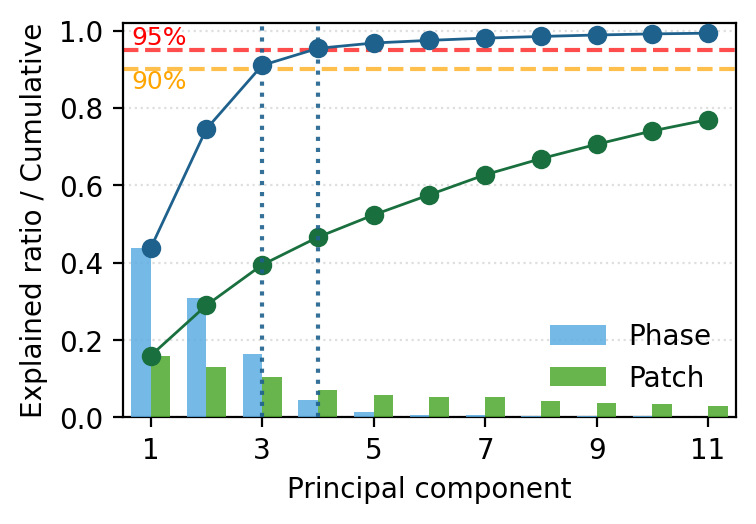
\includegraphics[width=\linewidth]{figures/etth1_pca_cycle_phase.png}
    \caption{PCA for tokens on \emph{ETTh1}.}
    \label{fig:pca_etth1}
  \end{subfigure}
  \hfill
  \begin{subfigure}[t]{0.32\textwidth}
    \centering
    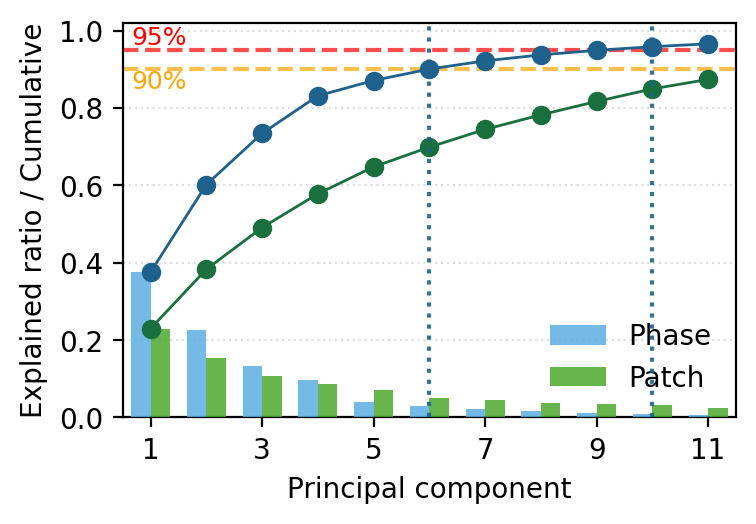
\includegraphics[width=\linewidth]{figures/etth2_pca_cycle_phase.png}
    \caption{PCA for tokens on \emph{ETTh2}.}
    \label{fig:pca_etth2}
  \end{subfigure}
  \hfill
  \begin{subfigure}[t]{0.32\textwidth}
    \centering
    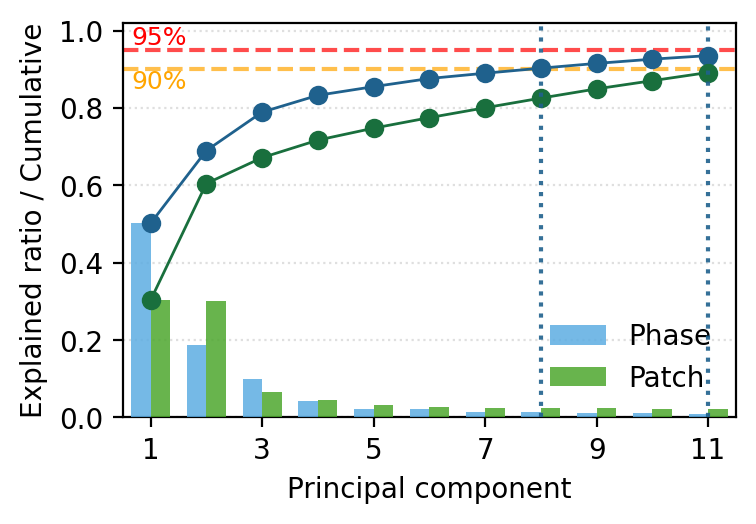
\includegraphics[width=\linewidth]{figures/ettm1_pca_cycle_phase.png}
    \caption{PCA for tokens on \emph{ETTm1}.}
    \label{fig:pca_ettm1}
  \end{subfigure}

  \vskip\baselineskip
  % 第二行
  \begin{subfigure}[t]{0.32\textwidth}
    \centering
    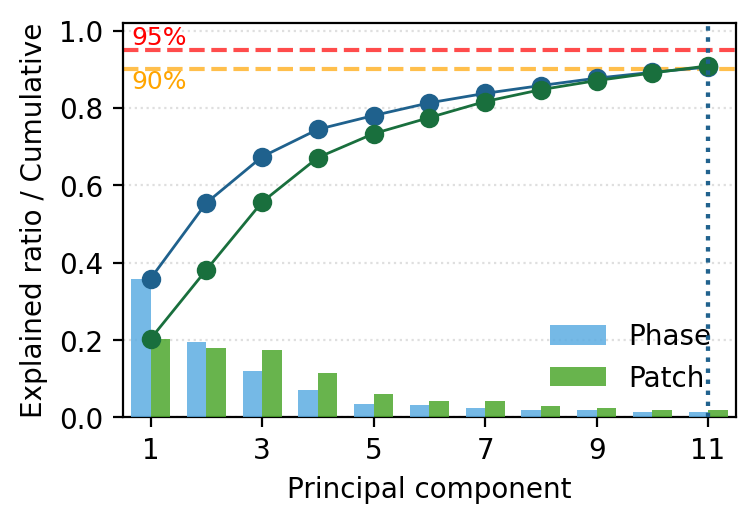
\includegraphics[width=\linewidth]{figures/ettm2_pca_cycle_phase.png}
    \caption{PCA for tokens on \emph{ETTm2}.}
    \label{fig:pca_ettm2}
  \end{subfigure}
  \hfill
  \begin{subfigure}[t]{0.32\textwidth}
    \centering
    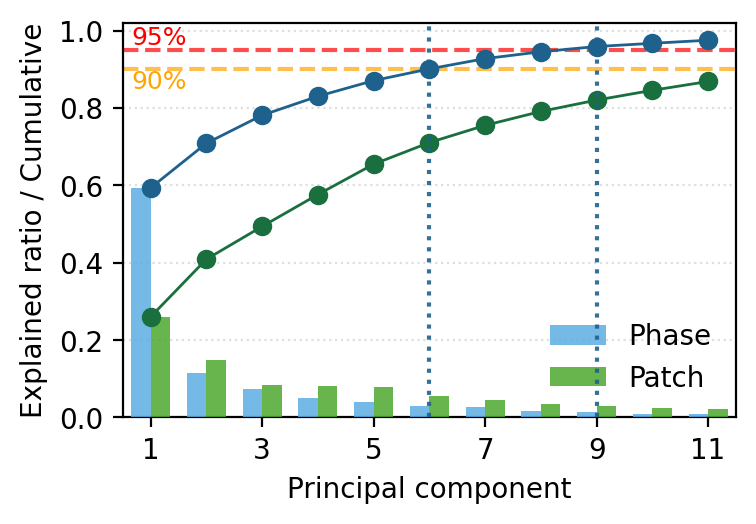
\includegraphics[width=\linewidth]{figures/electricity_pca_cycle_phase.png}
    \caption{PCA for tokens on \emph{Electricity}.}
    \label{fig:pca_ecl}
  \end{subfigure}
  \hfill
  \begin{subfigure}[t]{0.32\textwidth}
    \centering
    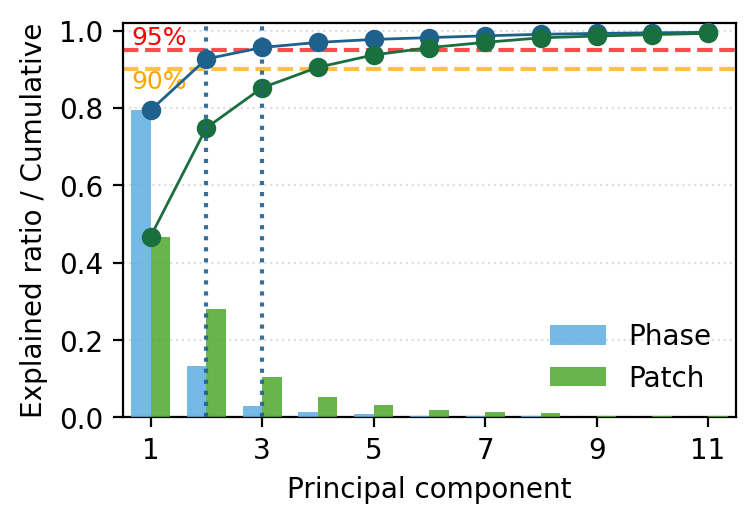
\includegraphics[width=\linewidth]{figures/weather_pca_cycle_phase.png}
    \caption{PCA for tokens on \emph{Weather}.}
    \label{fig:pca_weather}
  \end{subfigure}

  \caption{Visualization of phase tokenization across six datasets: ETTh1, ETTh2, ETTm1, ETTm2, Electricity, and Weather.}
  \label{fig:phase_token_comparison_detailed}
\end{figure*}

\revised{
\subsubsection{Comparison with Time Series Foundation Models}

To contextualize the performance of our approach, we compare \sysname against several representative foundation models drawn from the GIFT-Eval benchmark suite \citep{aksu2024giftevalbenchmarkgeneraltime}. 
Specifically, we include Chronos~\citep{ansari2024chronos}, Moirai~\citep{woo2024moirai}, and the recently released Moirai-2~\citep{liu2025moirai2} as baseline models.

Due to space limitations, we report results on the Web/DevOps subsets of the benchmark in \tabref{tab:model_mse_comparison}. 
These Web/DevOps datasets are \textit{not} well-studied by many existing works~\citep{nie2023patchtst, zhang2023crossformer, huang2025timebase, fits2024, lin2024sparsetsf}. 
Their heterogeneous and highly non-stationary behaviors make them particularly challenging, and thus provide a realistic environment to evaluate the generalization capability of large time series foundation models.

Beyond demonstrating strong overall competitiveness, the empirical results clearly highlight the 
unique strengths of phase-based representation in handling 
\emph{high-variance, noise-heavy workload patterns}. 
In particular, \sysname consistently outperforms all foundation-model baselines on the \texttt{bitbrains\_rnd} and \texttt{bitbrains\_fast\_storage} datasets—-two challenging subsets in GIFT-Eval due to frequent spikes and abrupt intensity shifts.
These results indicate that \sysname's phase-aware design provides substantially improved robustness and stability under highly volatile real-world workload traces, where traditional architecture tend to degrade.
}

\revised{
\begin{table*}[t]
\centering
\caption{Comparison of MSE (Mean) Across Four Forecasting Models on Web/CloudOps Datasets provided in GIFT-Eval.}
\label{tab:model_mse_comparison}
\footnotesize
\begin{tabular}{lcccc|c}
\hline
\textbf{Dataset} & \textbf{\sysname} & \textbf{Moirai-2} & \textbf{Moirai-base} & \textbf{Chronos-base} & \textbf{Best Model} \\
\hline
bizitobs\_l2c/5T/short           & 39.4347      & \textbf{20.6240}   & 22.1000        & 24.1000        & Moirai-2 \\
bizitobs\_l2c/H/short            & 99.9582      & \textbf{67.8501}   & 272.0000       & 243.0000       & Moirai-2 \\
bitbrains\_rnd/H/short           & \textbf{1,970,330} & 2,235,573     & 4,020,000      & 2,210,000      & \sysname \\
bitbrains\_rnd/5T/short          & \textbf{1,606,034} & 1,660,532     & 180,000,000    & 1,800,000      & \sysname \\
bizitobs\_application/10S/short  & 4,653,132    & \textbf{621,852}   & 6,360,000      & 6,030,000      & Moirai-2 \\
bitbrains\_fast\_storage/H/short & \textbf{2,585,180}    & 2,942,651          & 604,000,000    & 2,620,000 & \sysname \\
bitbrains\_fast\_storage/5T/short& \textbf{1,887,398} & 2,142,125     & 25,400,000,000 & 1,920,000      & \sysname \\
bizitobs\_service/10S/short      & 26,523       & \textbf{4,798}     & 51,900         & 37,100         & Moirai-2 \\
\hline
\end{tabular}
\end{table*}
}




\subsection{Additional Hyper Parameters Analysis}
\subsubsection{Impact of Model Parameter Scale on Performance}
We conducted comparative experiments on three variants of the \sysname model with different parameter scales across the Electricity, Traffic, and Weather datasets. The three configurations are: a single-layer model with latent dimension 8 ($\approx$1.72K parameters), a single-layer model with latent dimension 16 ($\approx$5.48K parameters), and a two-layer model with latent dimension 32 ($\approx$37.1K parameters). \figref{tab:phaseformer_params_variants} summarizes the results in terms of MSE, MAE and FLOPs.

Overall, the effect of model scale on performance is not consistent. On the Traffic dataset, larger models yield slight improvements, whereas on the Electricity and Weather datasets, the smaller and medium-sized models perform better. These findings indicate that \sysname achieves a favorable balance between computational efficiency and predictive accuracy at relatively small parameter scales, and increasing model size does not lead to uniform gains across all tasks.

\begin{table*}[t]
\centering
\caption{Comparison of \sysname variants. Each cell reports MSE, MAE, and FLOPs. The input length is fixed as 720 steps and the output length is fixed as 96 steps. The best results are marked with \best{Bold}, and the second-best results are marked with \second{Underlined}.}
\label{tab:phaseformer_params_variants}
\small  % 或者 \footnotesize, \scriptsize
\begin{tabular}{c|ccc|ccc|ccc}
\hline
\multirow{2}{*}{Dataset}
& \multicolumn{3}{c|}{\textbf{\sysname-1.7K}} 
& \multicolumn{3}{c|}{\textbf{\sysname-5K}} 
& \multicolumn{3}{c}{\textbf{\sysname-37K}} \\
\cline{2-10}
& MSE & MAE & FLOPs
& MSE & MAE & FLOPs
& MSE & MAE & FLOPs \\
\hline
Electricity 
& \best{0.129} & \best{0.220} & \best{9.41M}
& \best{0.129} & \second{0.221} & \second{31.97M}
& \second{0.131} & \second{0.223} & 221.05M \\
Traffic     
& \second{0.361} & \second{0.241} & \best{25.27M}
& 0.366 & 0.243 & \second{85.84M}
& \best{0.360} & \best{0.236} & 593.61M \\
Weather     
& \best{0.150} & \second{0.199} & \best{0.62M}
& \second{0.151} & \best{0.194} & \second{2.09M}
& 0.174 & 0.217 & 14.46M \\
\hline
\end{tabular}
\end{table*}

\subsubsection{Impact of Input Length on Performance}

We examine how the input window size affects the prediction accuracy and computational cost of \sysname. 
Throughout this section, $L$ denotes using the most recent $L$ time steps as model input. The output length is fixed as 96 steps.
As summarized in ~\figref{fig:input_length_prediction_errors}, increasing $L$ reduces MSE and MAE across datasets, indicating that \sysname benefits from longer historical context for modeling long-range temporal dependencies.

In terms of efficiency, the parameter count and FLOPs per forward pass remain nearly constant as $L$ increases, with only modest growth (see ~\figref{fig:input_length_efficiency}) attributable primarily to the embedding stage. 
This behavior arises because the sequence length processed by the core encoder/decoder is governed by the number of \emph{phases}, which depends on the data’s learned periodic structure rather than by the raw input length.
Consequently, scaling $L$ mainly affects the embedding computations, whose cost is relatively small compared to the phase-based modules.

\begin{figure*}[htbp]
    \centering
    % 子图1: Electricity
    \begin{subfigure}[b]{0.32\textwidth}
        \centering
        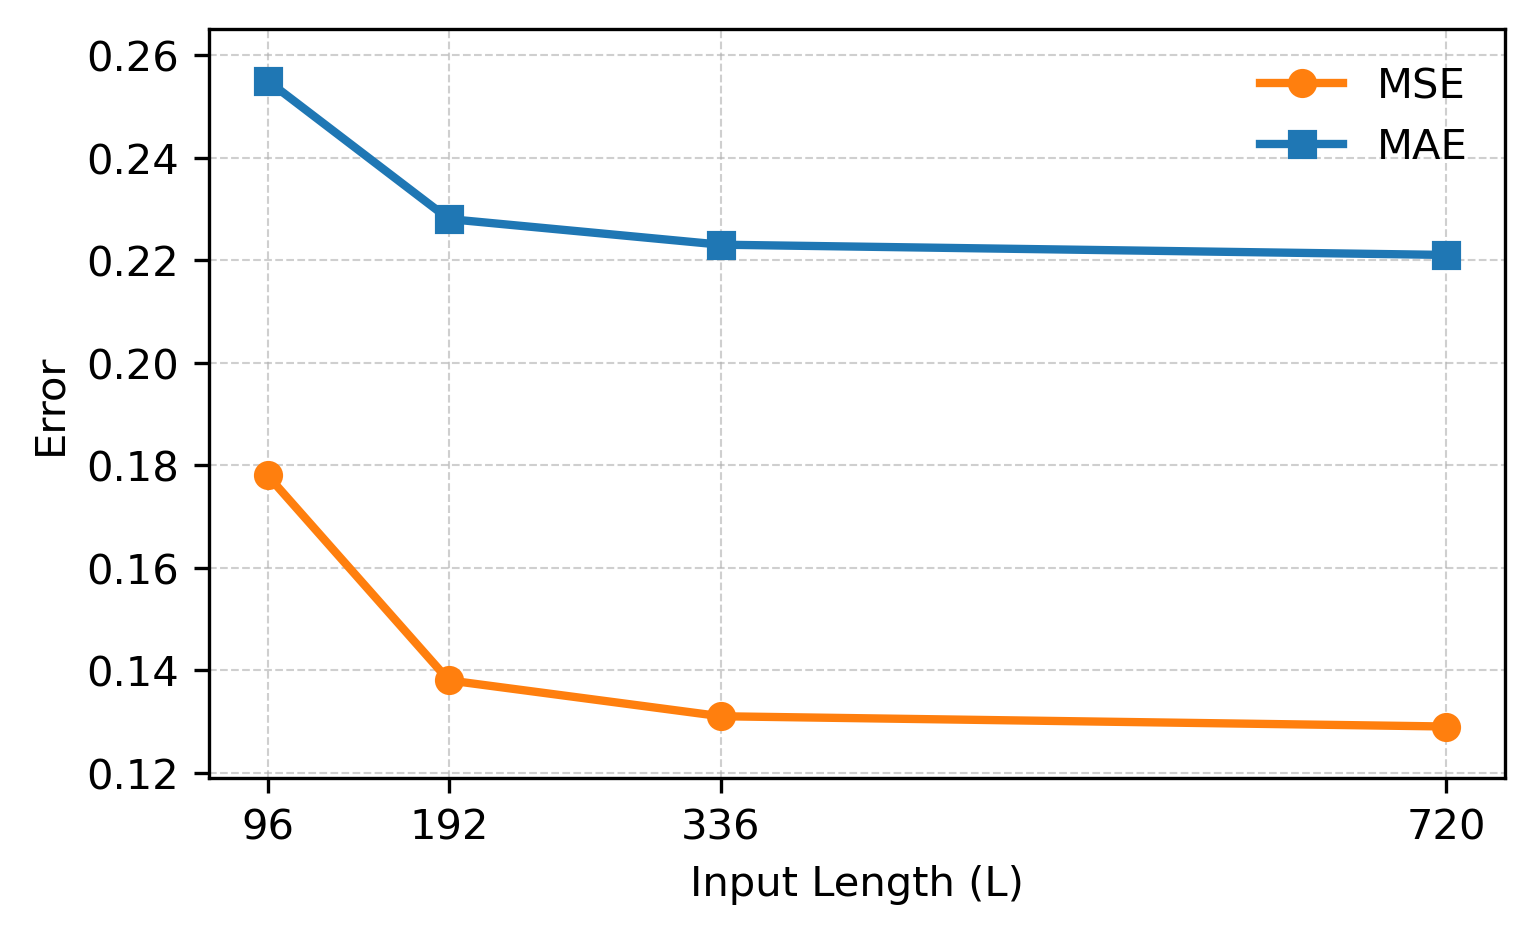
\includegraphics[width=\textwidth]{figures/performance_electricity.png}
        \caption{Electricity}
    \end{subfigure}
    % 子图2: Traffic
    \begin{subfigure}[b]{0.32\textwidth}
        \centering
        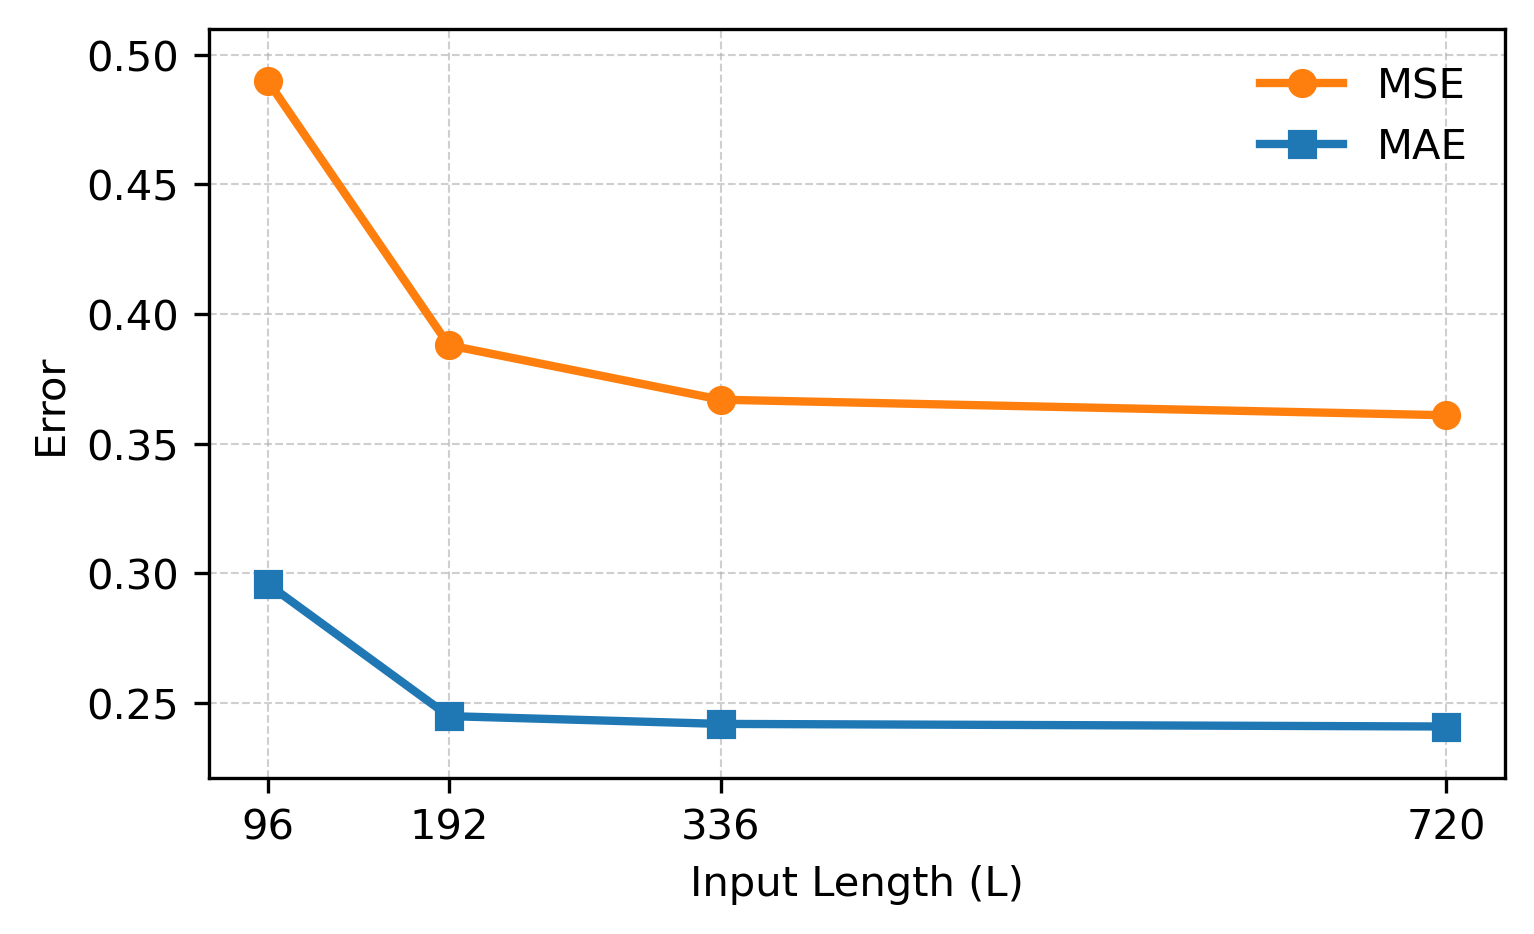
\includegraphics[width=\textwidth]{figures/performance_traffic.png}
        \caption{Traffic}
    \end{subfigure}
    % 子图3: Weather
    \begin{subfigure}[b]{0.32\textwidth}
        \centering
        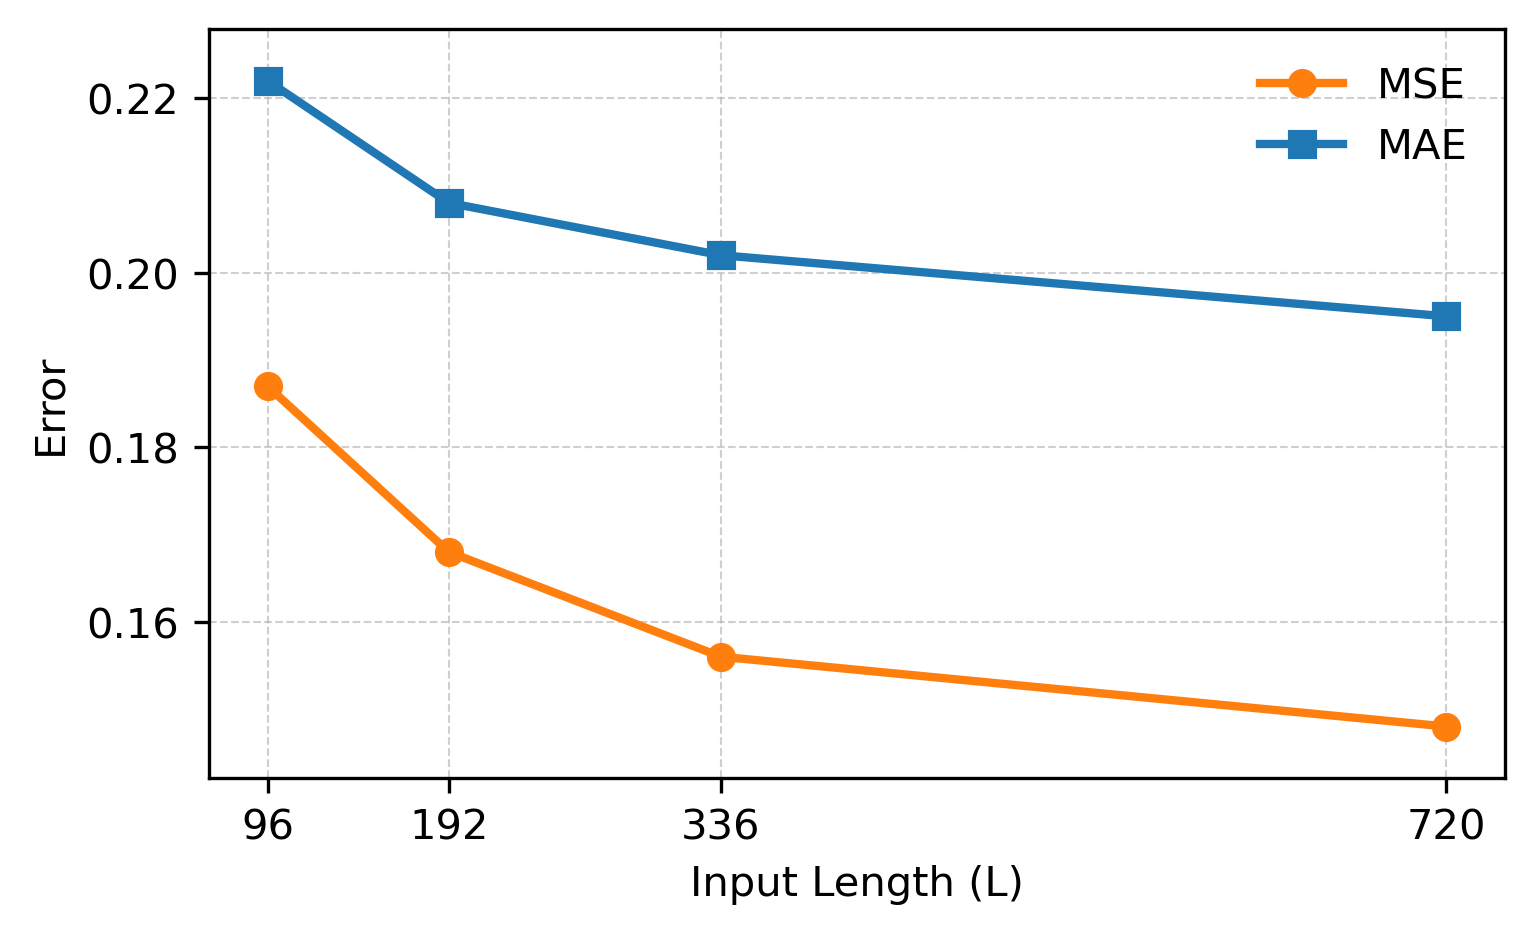
\includegraphics[width=\textwidth]{figures/performance_weather.png}
        \caption{Weather}
    \end{subfigure}

    \caption{Prediction error test results across datasets under different input lengths.}
    \label{fig:input_length_prediction_errors}
\end{figure*}

\begin{figure*}[htbp]
    \centering
    % 子图1: Electricity
    \begin{subfigure}[b]{0.32\textwidth}
        \centering
        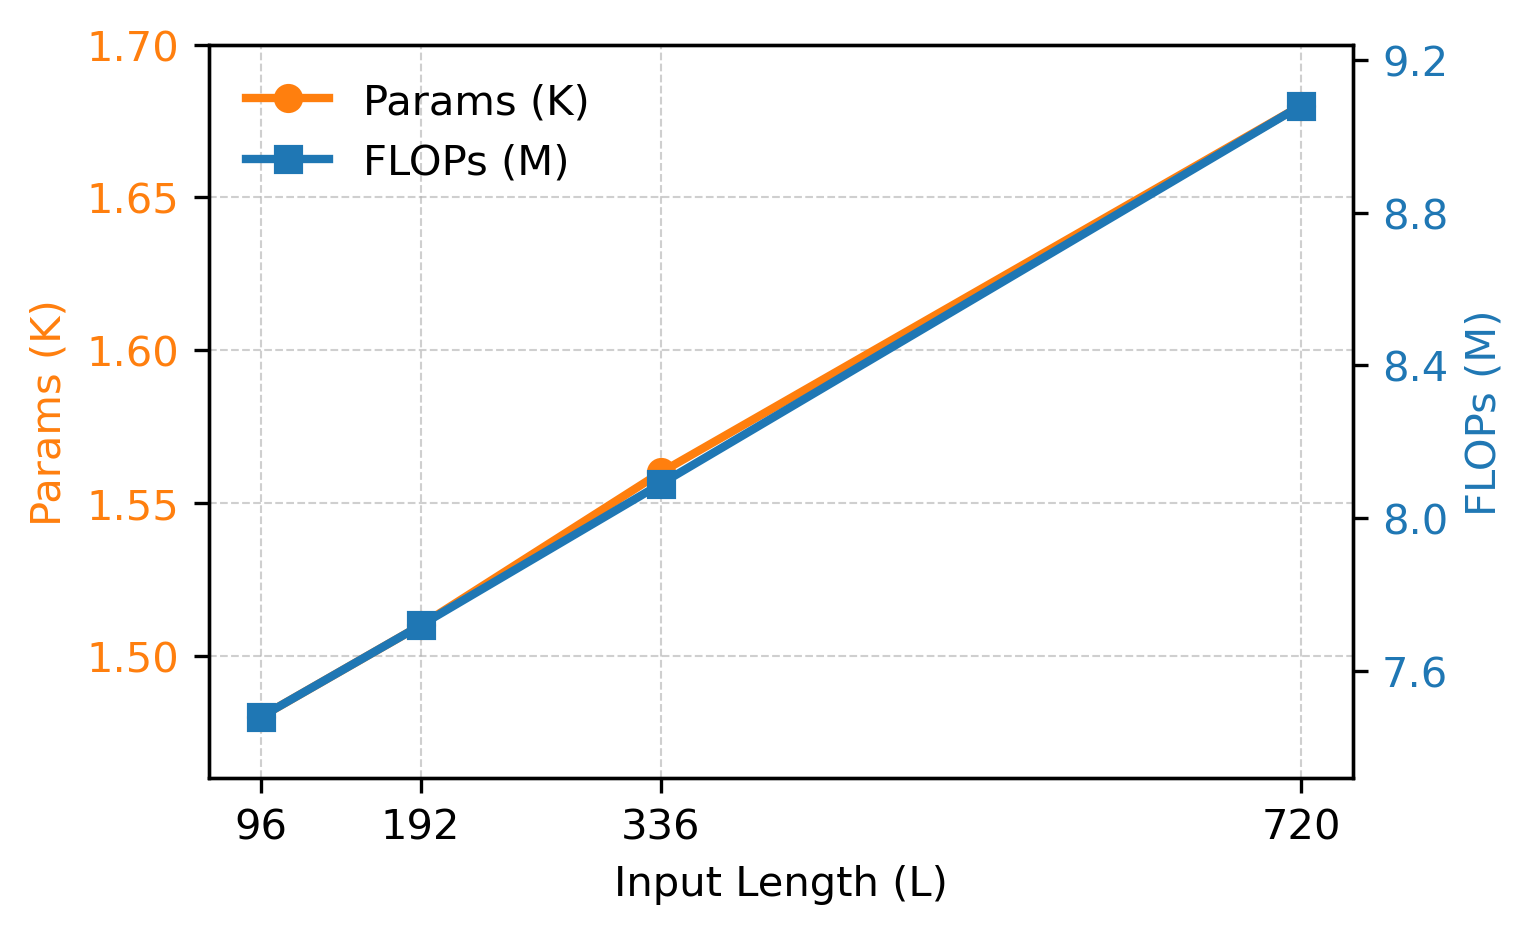
\includegraphics[width=\textwidth]{figures/efficiency_electricity.png}
        \caption{Electricity}
    \end{subfigure}
    % 子图2: Traffic
    \begin{subfigure}[b]{0.32\textwidth}
        \centering
        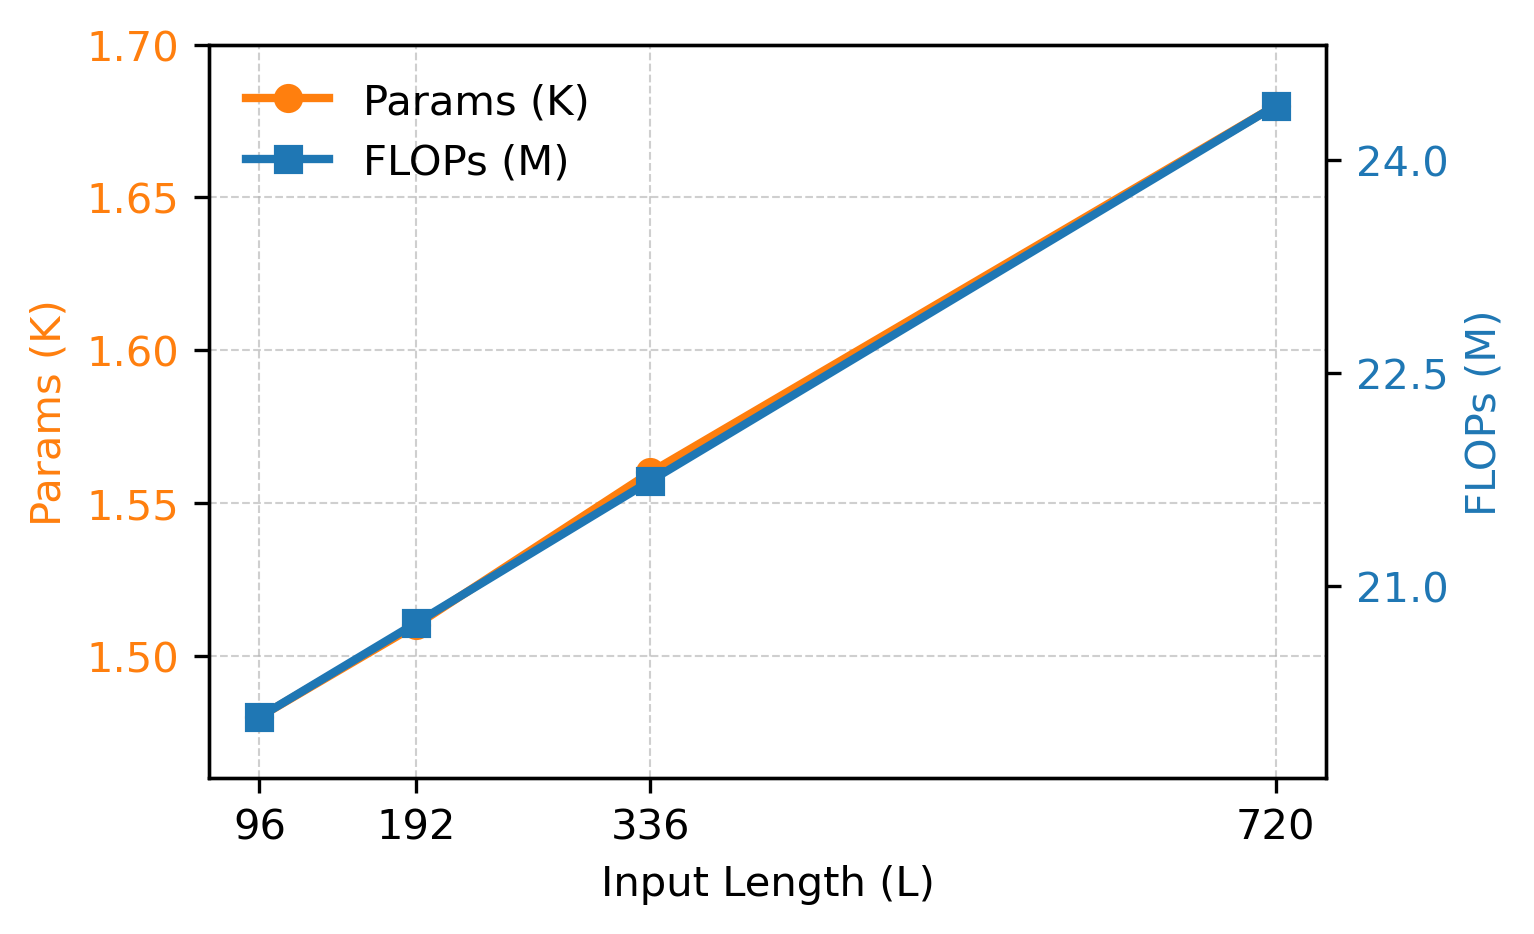
\includegraphics[width=\textwidth]{figures/efficiency_traffic.png}
        \caption{Traffic}
    \end{subfigure}
    % 子图3: Weather
    \begin{subfigure}[b]{0.32\textwidth}
        \centering
        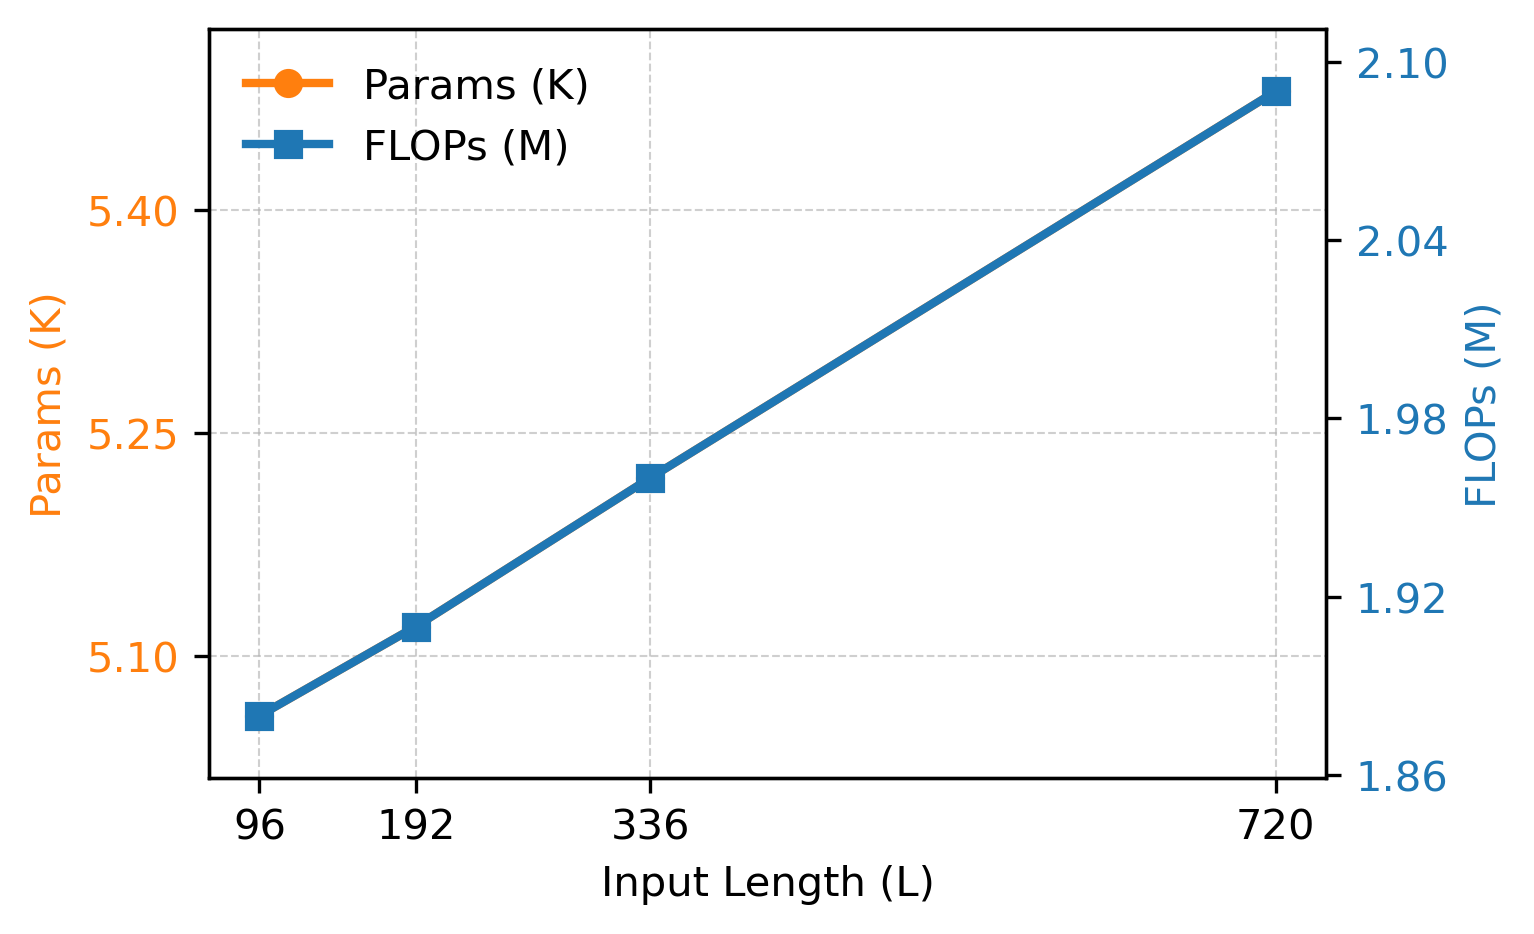
\includegraphics[width=\textwidth]{figures/efficiency_weather.png}
        \caption{Weather}
    \end{subfigure}

    \caption{Efficiency evaluation of \sysname\ across datasets with varying input lengths.}
    \label{fig:input_length_efficiency}
\end{figure*}

\revised{
\subsection{Analysis of Fine-Grained Temporal Information Retention}
To examine whether Phase Tokenization preserves essential intra-cycle dynamics after compressing periodic structures, we conduct a reconstruction experiment on the Traffic dataset. Given an input sequence of length 720, \sysname is trained to reconstruct sequences of the same length, removing forecasting uncertainty and isolating the representational capacity of the phase embeddings.

\fakeparagraph{Setup}
We evaluate the retention of fine-grained information by computing the reconstruction residual and analyzing it in both the time and frequency domains. In particular, we estimate the power spectral density (PSD) of the residual to detect whether certain frequency components, especially those associated with short-term or high-frequency dynamics, are systematically diminished.

\begin{figure*}
    \centering
    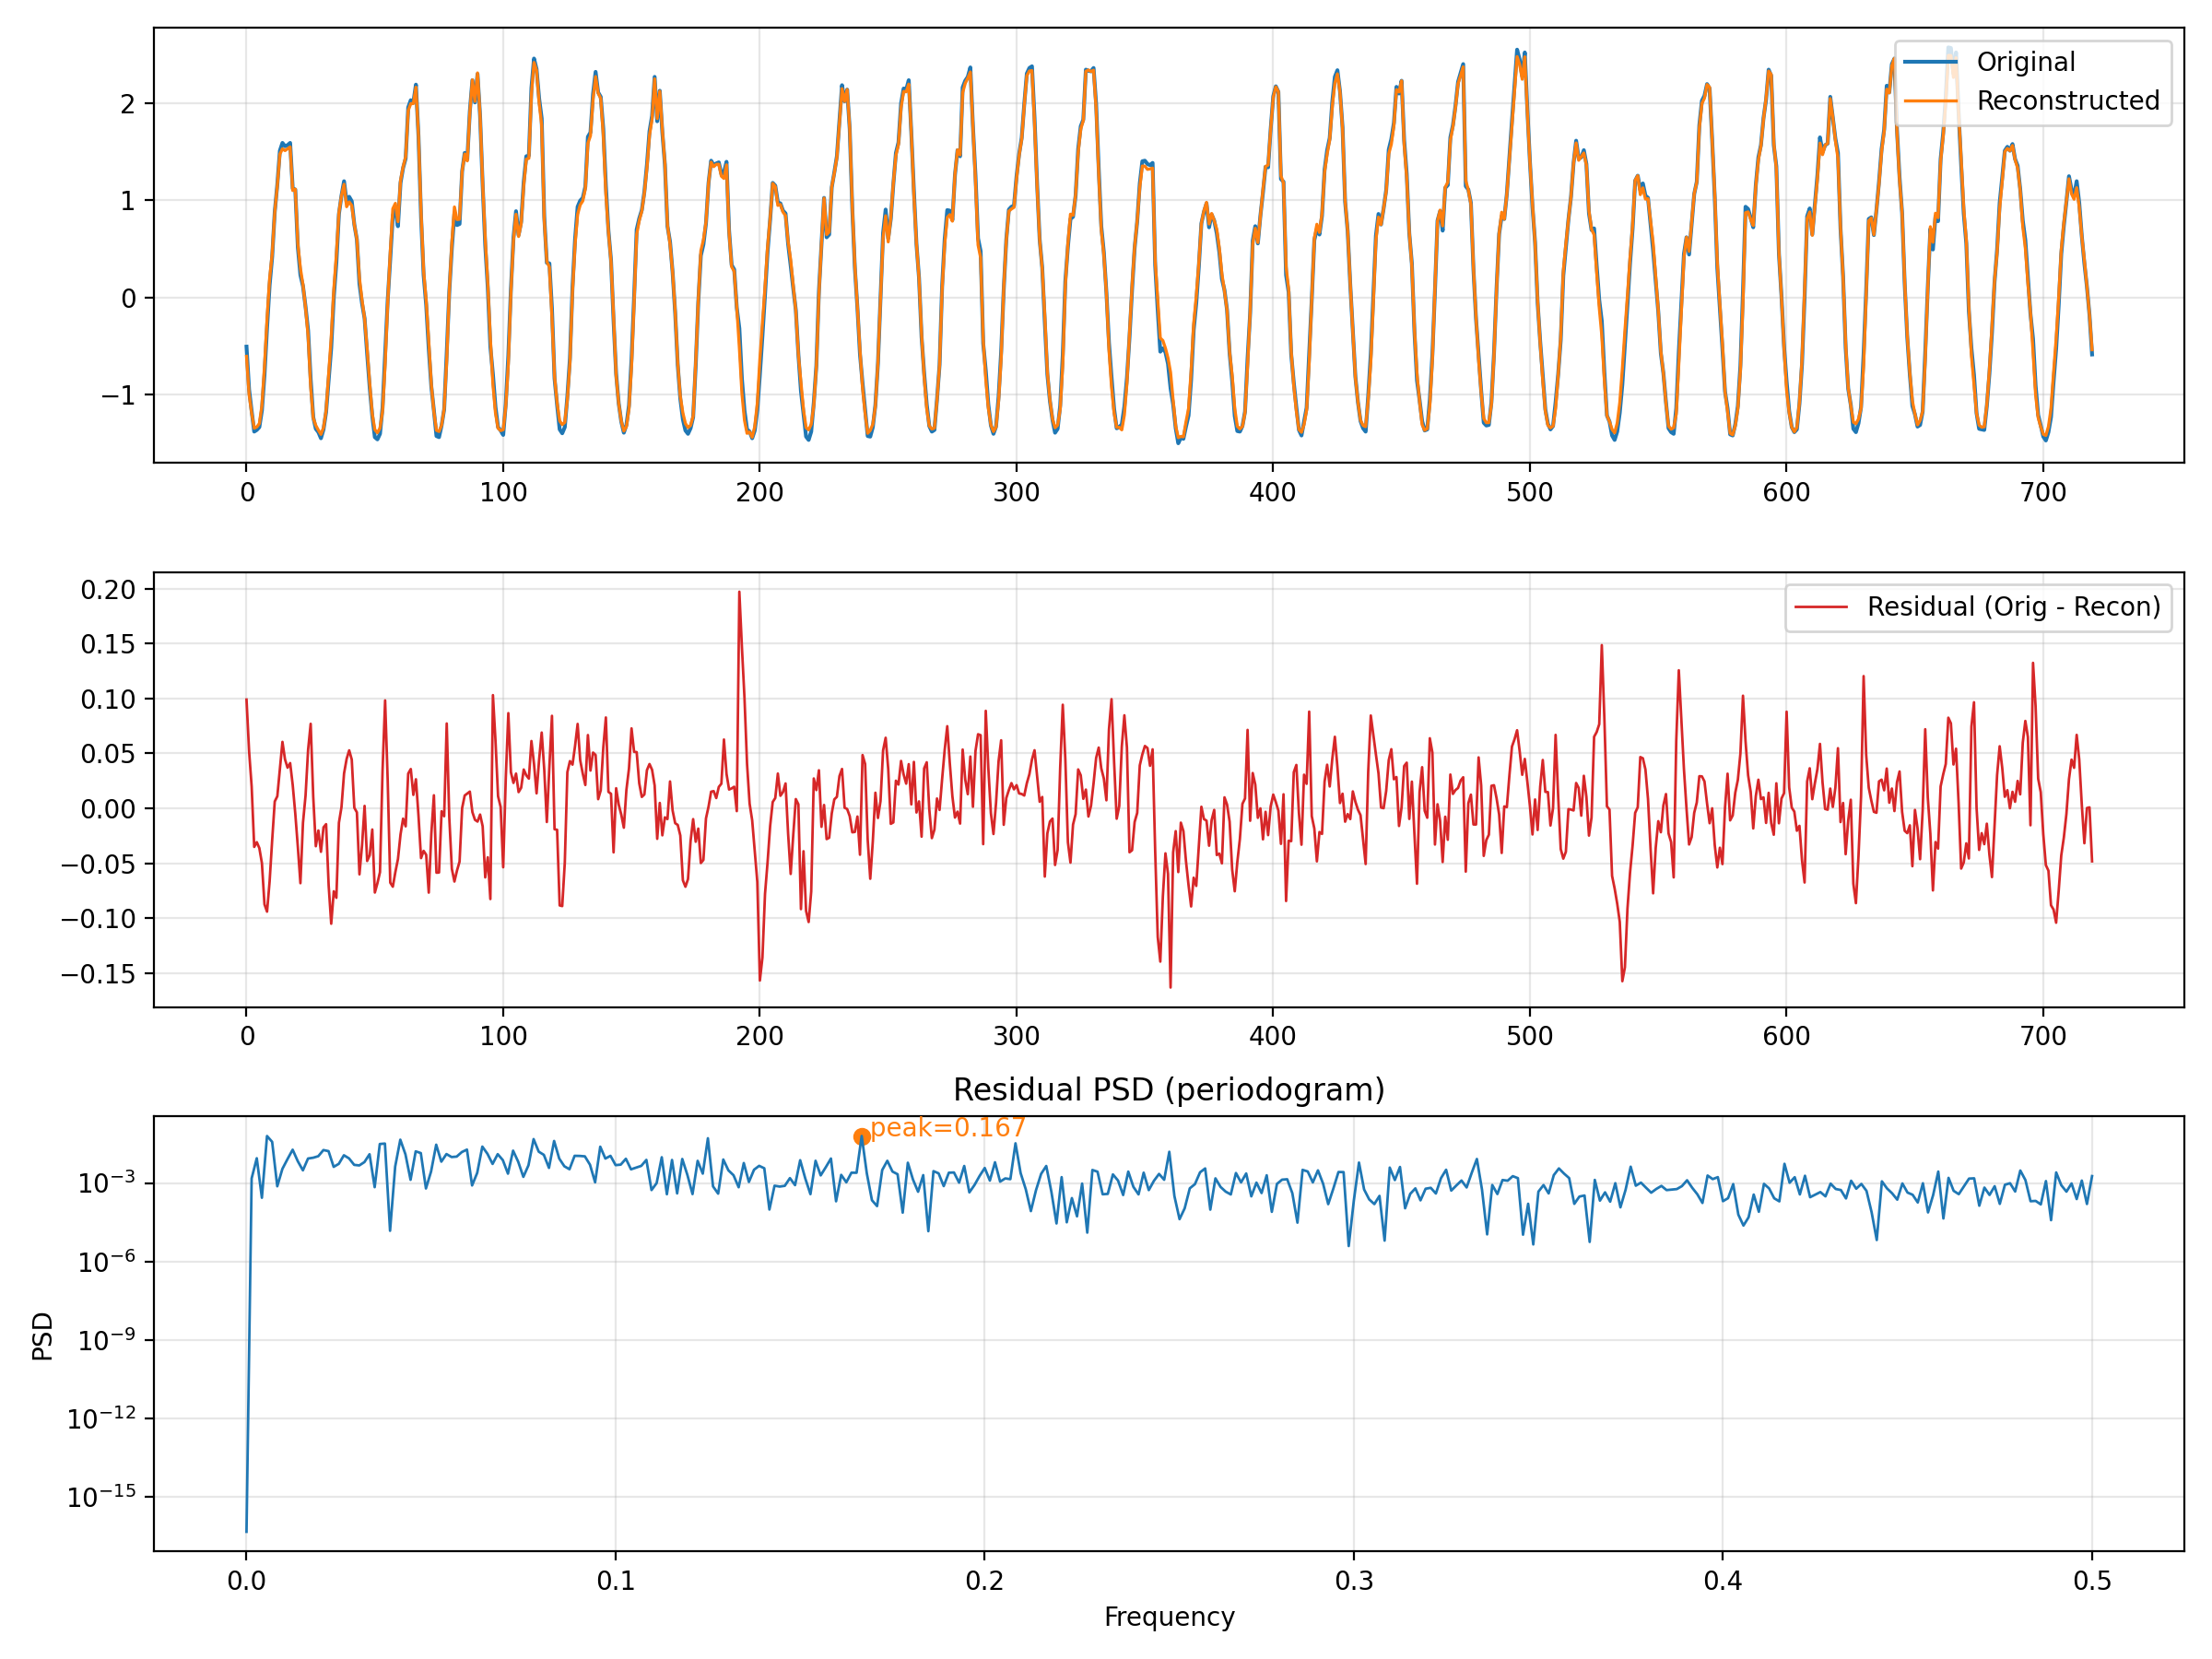
\includegraphics[width=0.75\textwidth]{figures/reconstruction_analysis.png}
    \caption{Time-domain and power-spectrum visualizations of the reconstruction residuals when \sysname reconstructs 720 input time steps on the Traffic dataset.}
    \label{fig:reconstruction_analysis}
\end{figure*}

\fakeparagraph{Frequency Analysis of the Residual}
The PSD analysis in \figref{fig:reconstruction_analysis} shows that residual energy is evenly distributed across the spectrum, with no noticeable concentration or suppression in any frequency band. This indicates that Phase Tokenization does not introduce frequency-dependent information loss. Despite compressing each cycle into a compact phase representation, the model retains the ability to capture fine-grained intra-cycle dynamics, supporting the effectiveness of phase-based temporal abstraction for long-sequence forecasting.
}



\subsection{Showcases}

To provide a clearer comparison of predictive performance across different models, we present the results of \sysname, PatchTST, FITS, and TimeBase on the Traffic dataset.
\sysname demonstrates strong predictive performance, as reflected by both the shape of its forecasts and the actual prediction errors.

Compared with \sysname, PatchTST produces lower peak values within each cycle, failing to fully match the true curve. This discrepancy is likely due to phase shifts in the periodic pattern that reduce peak amplitudes.
FITS, which performs prediction in the frequency domain with frequency band partitioning, tends to overlook high-frequency information. As a result, its predictions deviate from the ground truth, though the forecasts still preserve a periodic structure.
TimeBase aligns well with the general cyclical pattern but fails to capture true variations across cycles, a limitation stemming from its patch-based basis construction mechanism.


\begin{figure*}[t]
    \centering
    % 第一行
    \begin{subfigure}{0.47\textwidth}
        \centering
        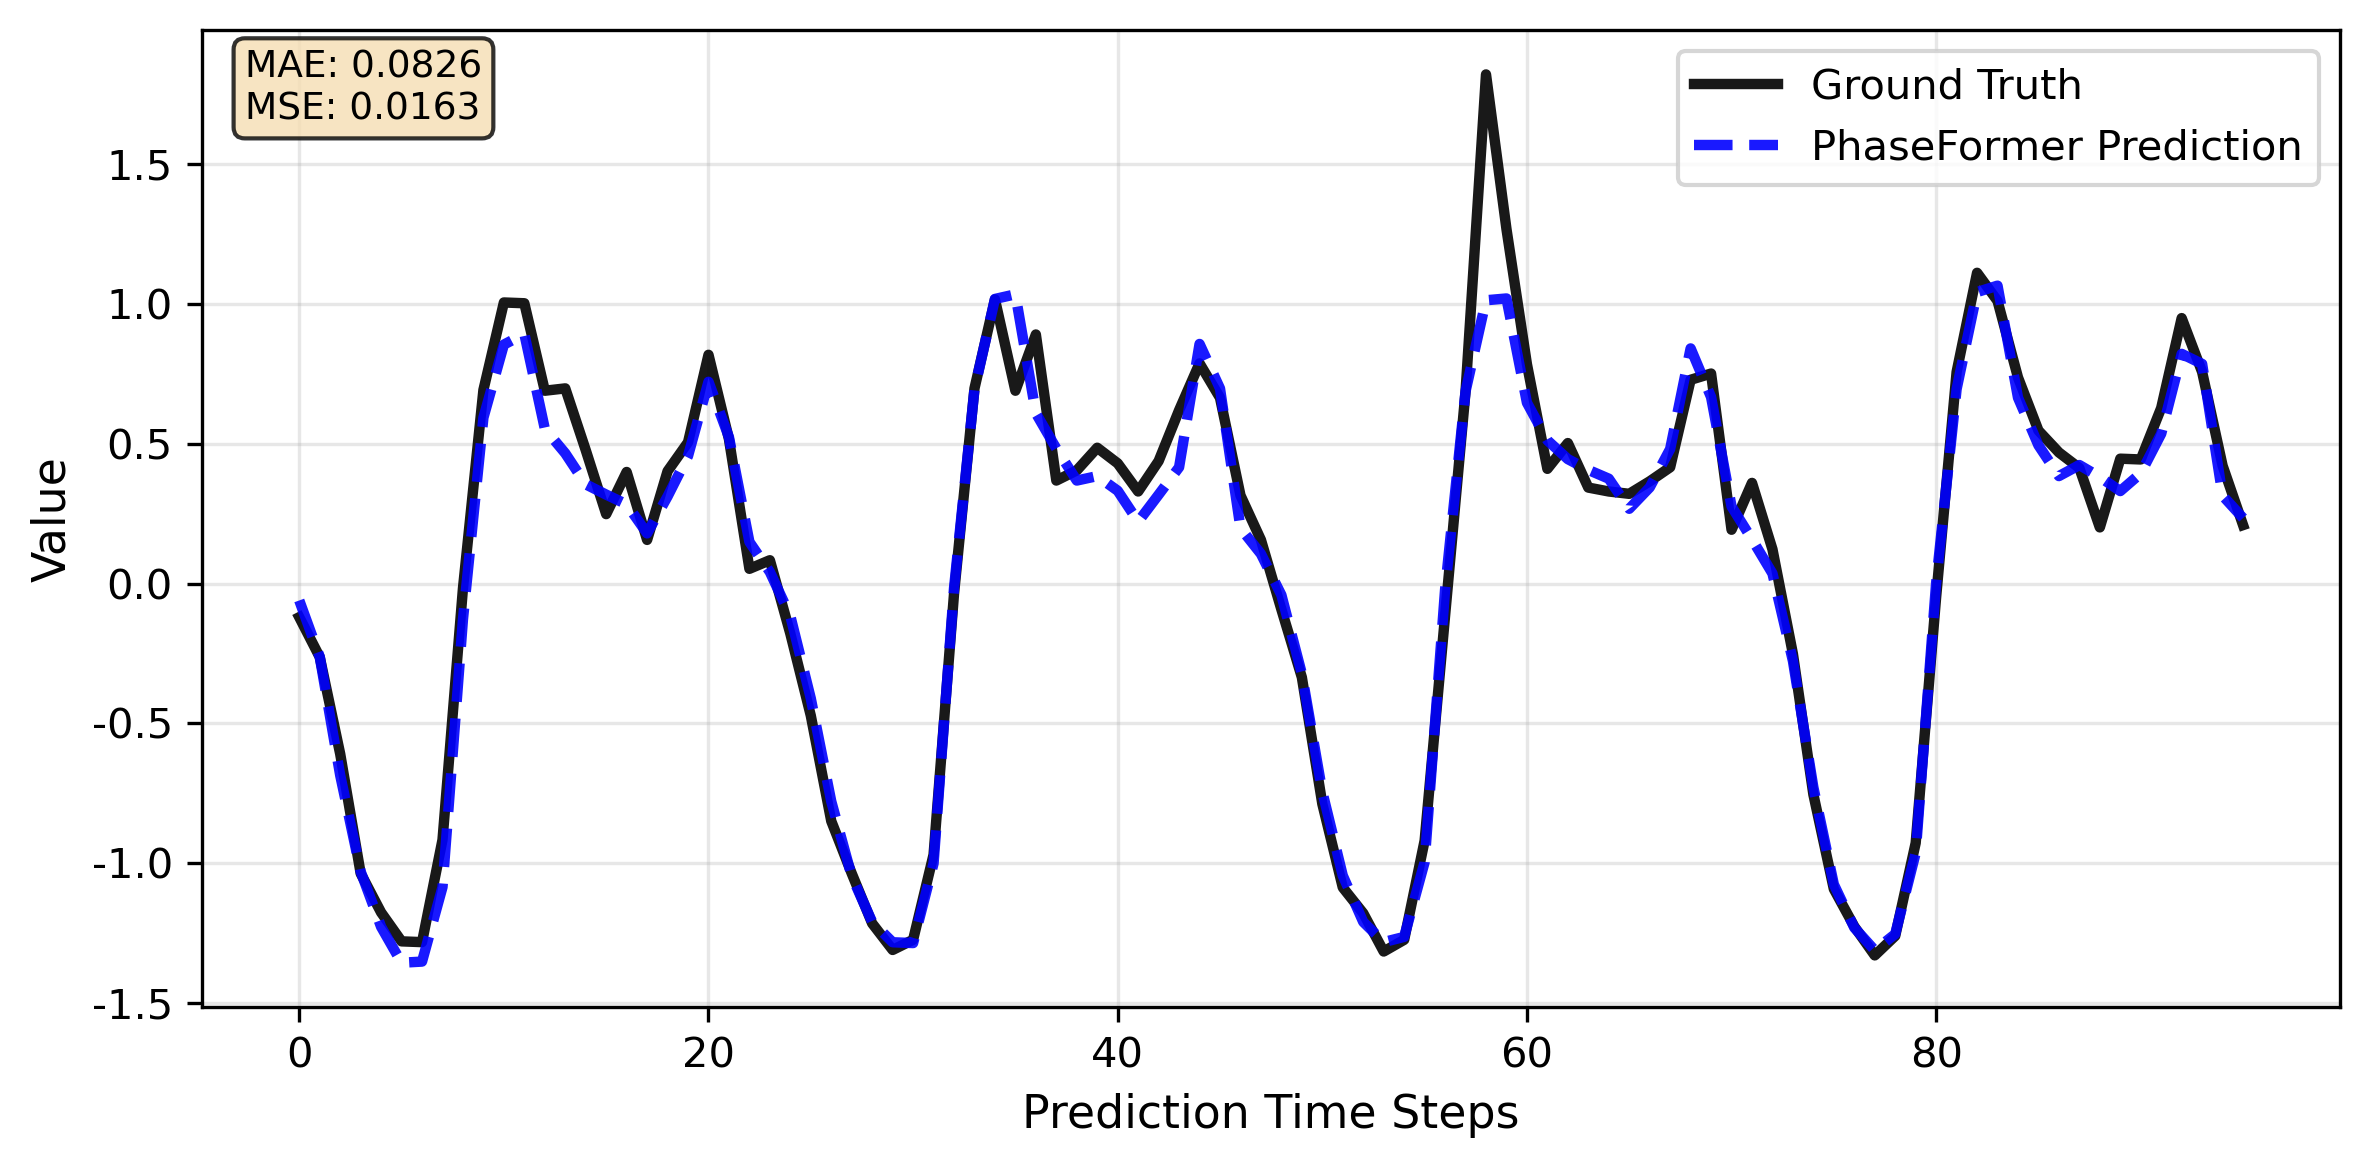
\includegraphics[width=\linewidth]{figures/PhaseFormer_prediction_20250923_021323.png}
        \caption{\sysname}
    \end{subfigure}
    \hfill
    \begin{subfigure}{0.47\textwidth}
        \centering
        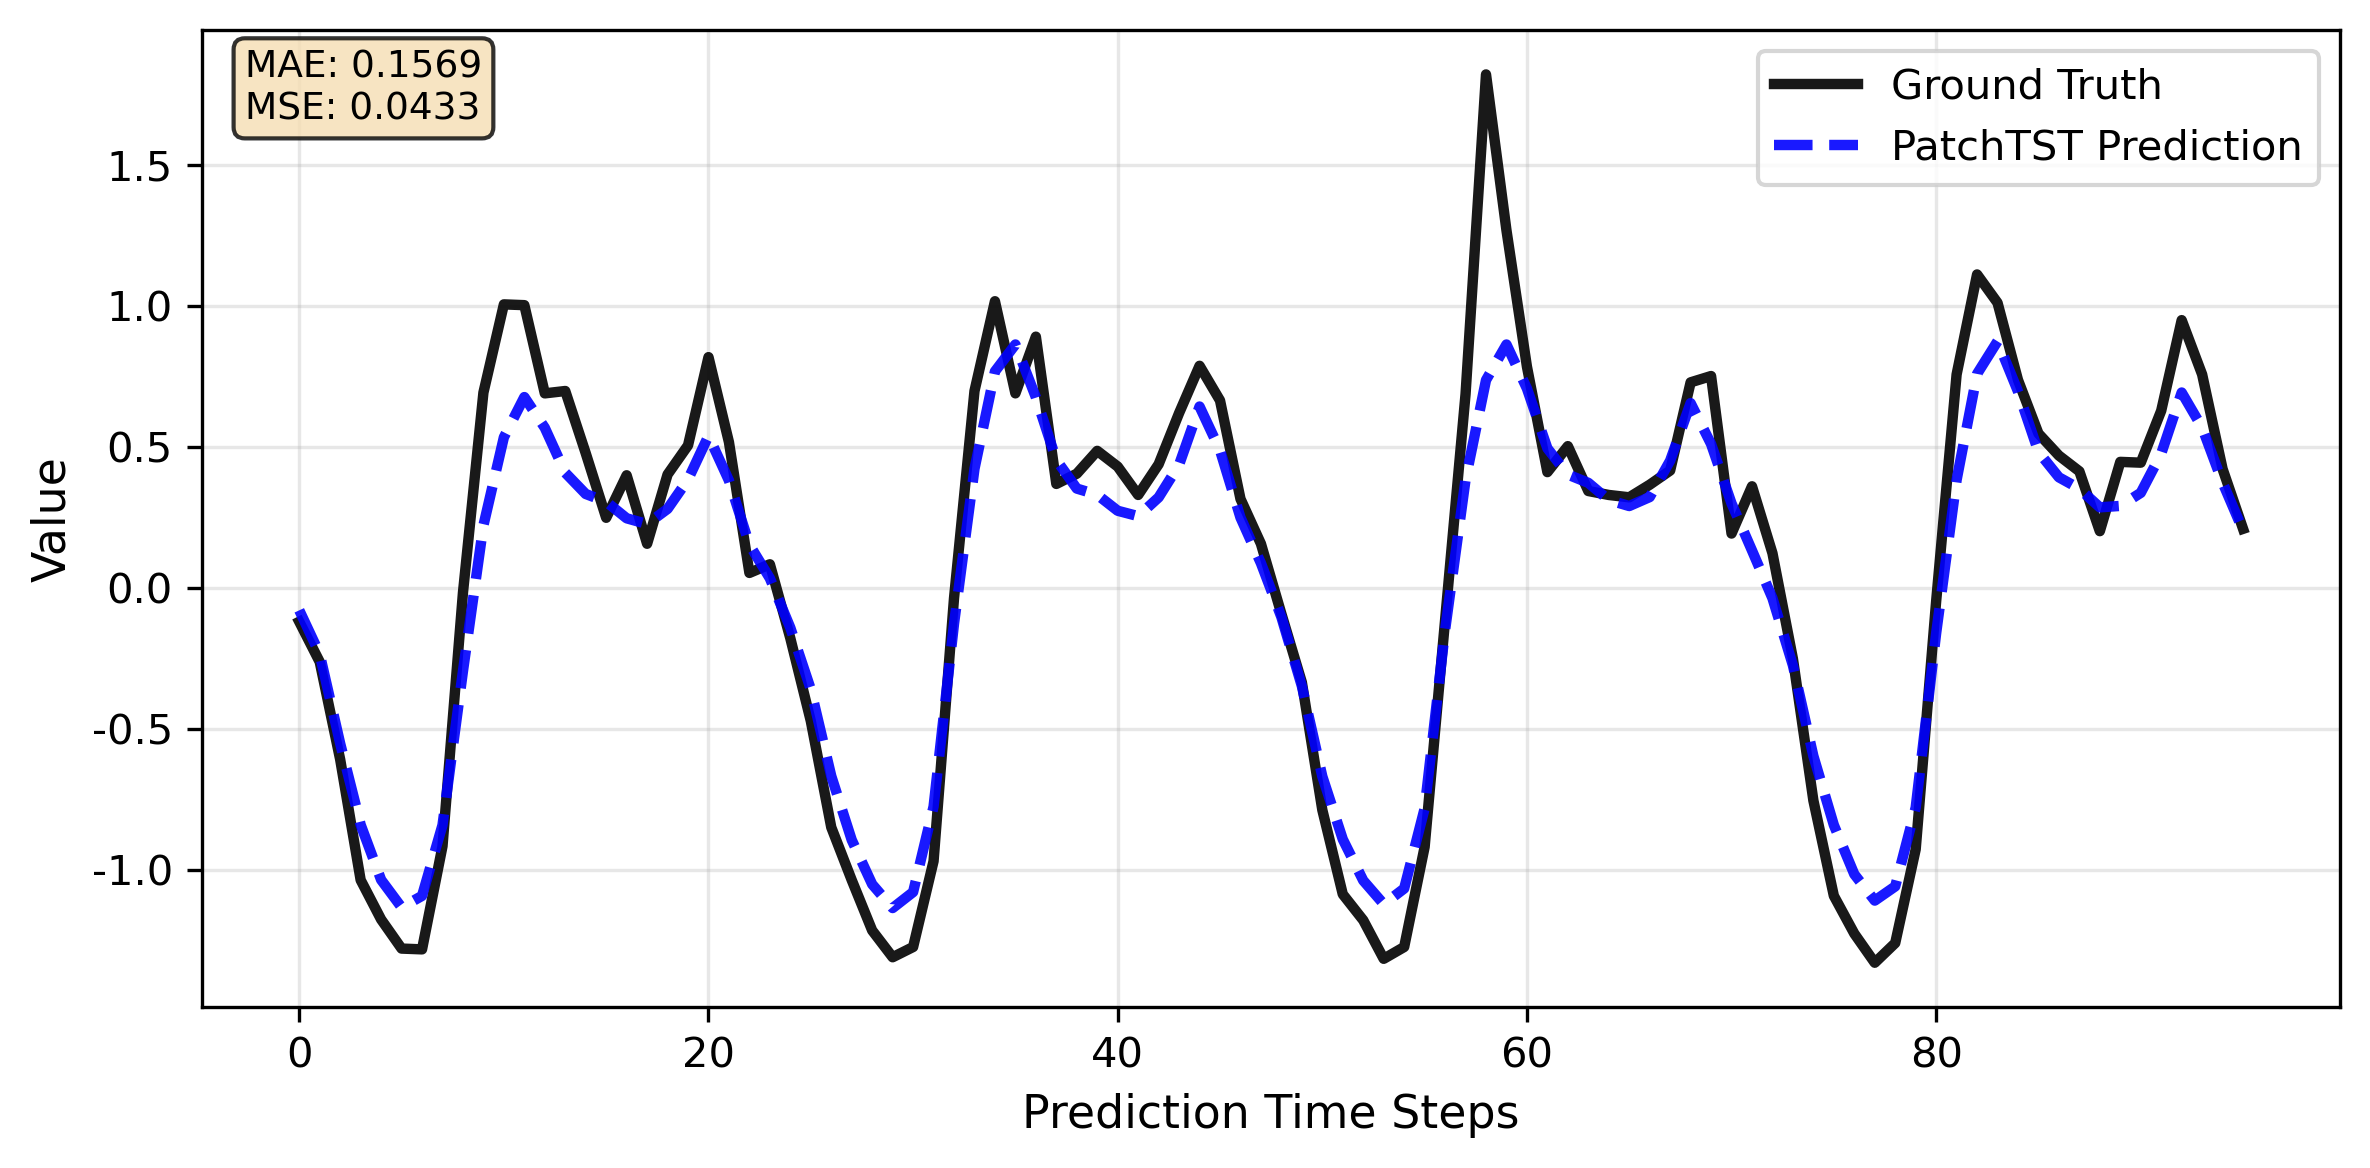
\includegraphics[width=\linewidth]{figures/PatchTST_prediction_20250923_021323.png}
        \caption{PatchTST}
    \end{subfigure}

    % 第二行
    \vskip\baselineskip
    \begin{subfigure}{0.47\textwidth}
        \centering
        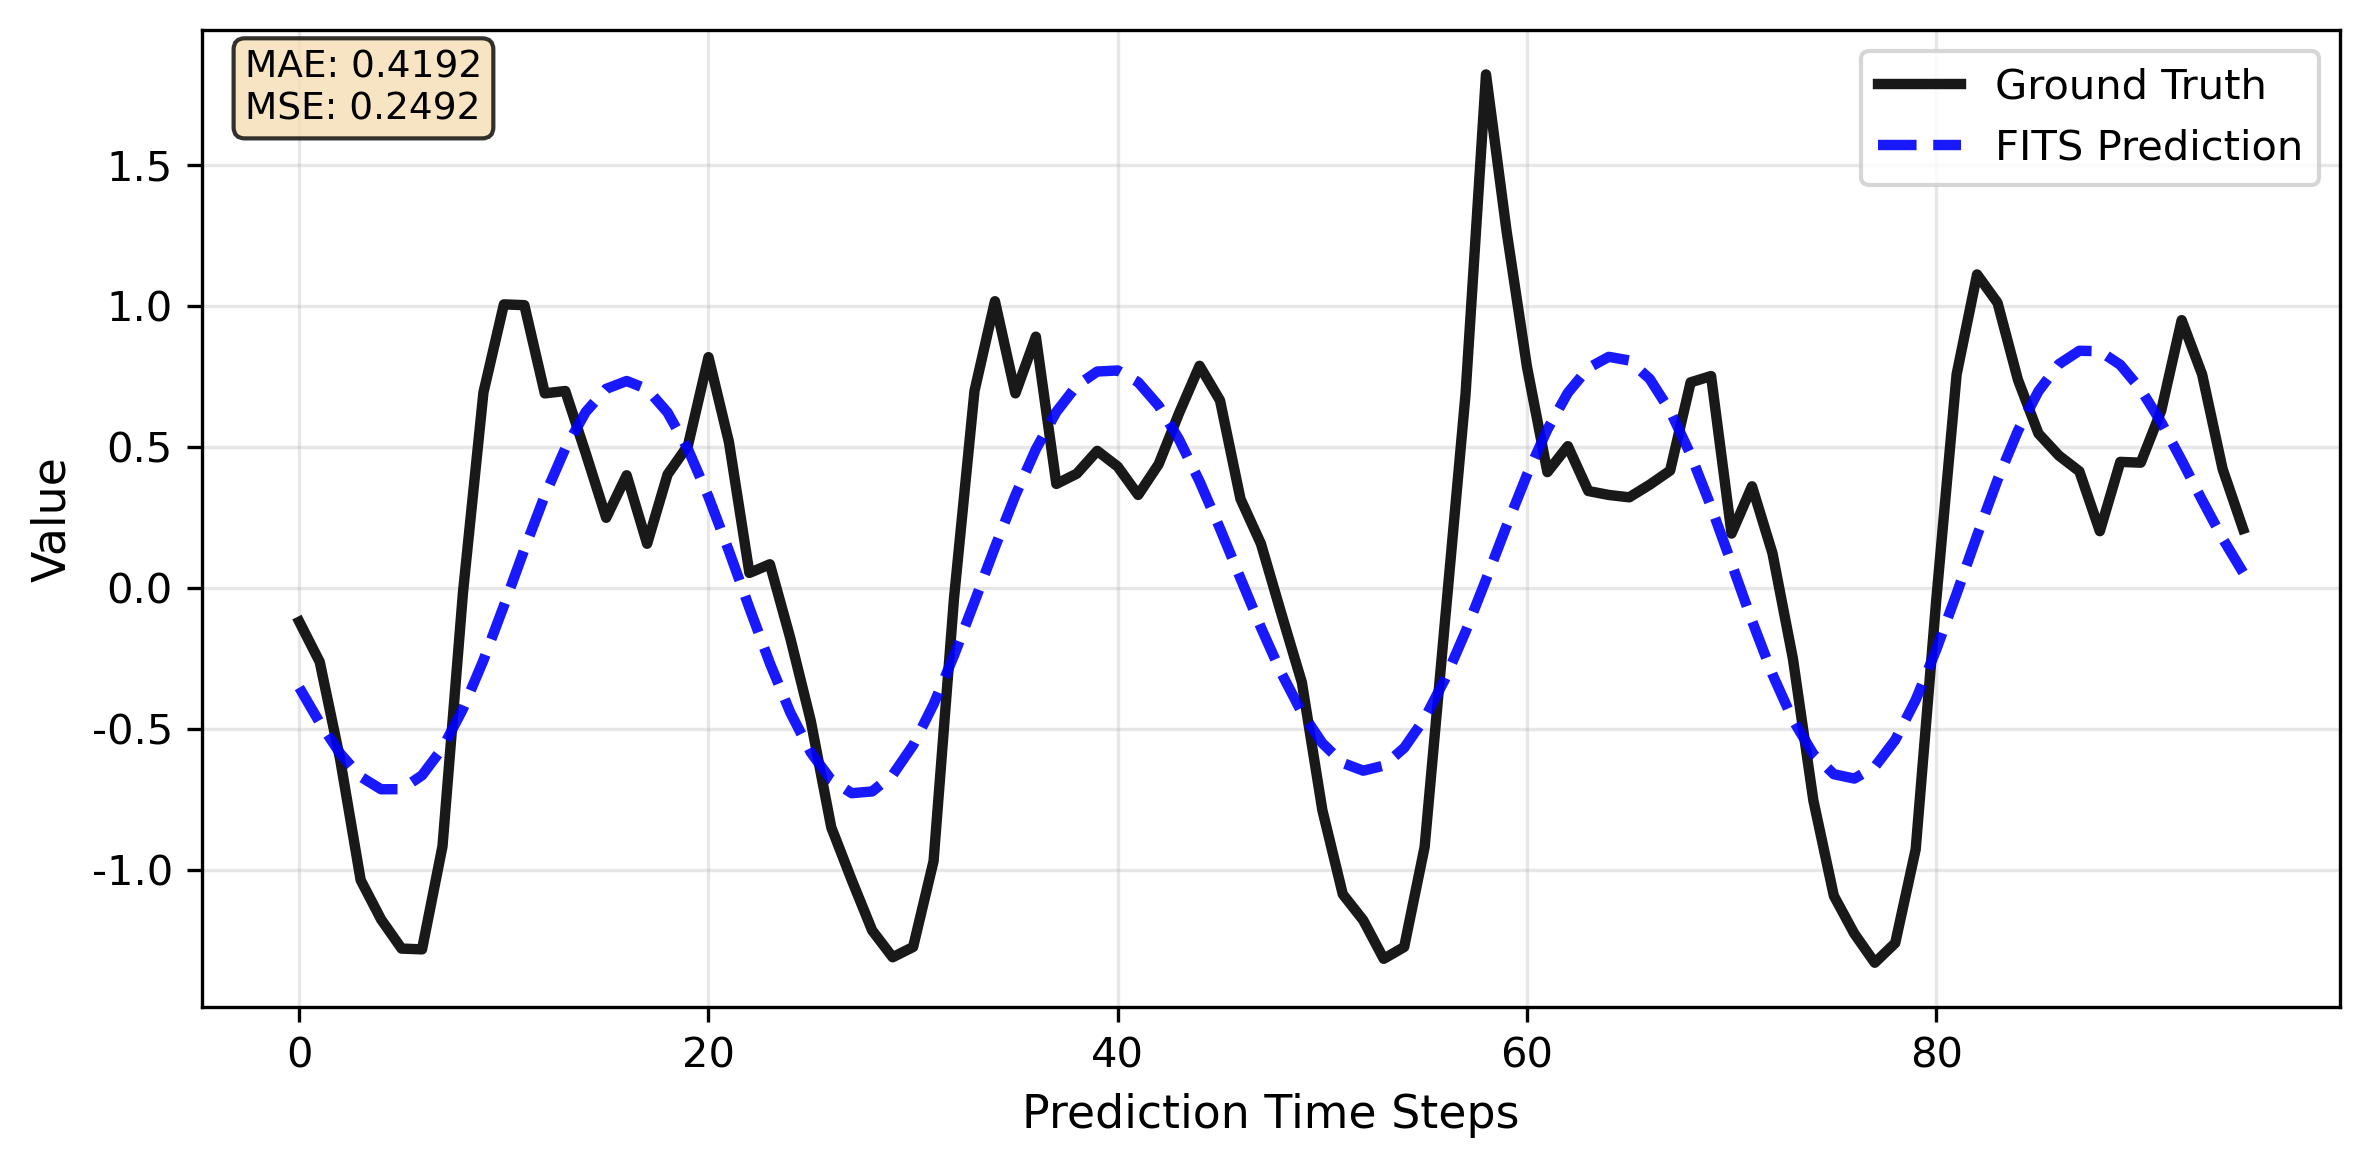
\includegraphics[width=\linewidth]{figures/FITS_prediction_20250923_021323.png}
        \caption{FITS}
    \end{subfigure}
    \hfill
    \begin{subfigure}{0.47\textwidth}
        \centering
        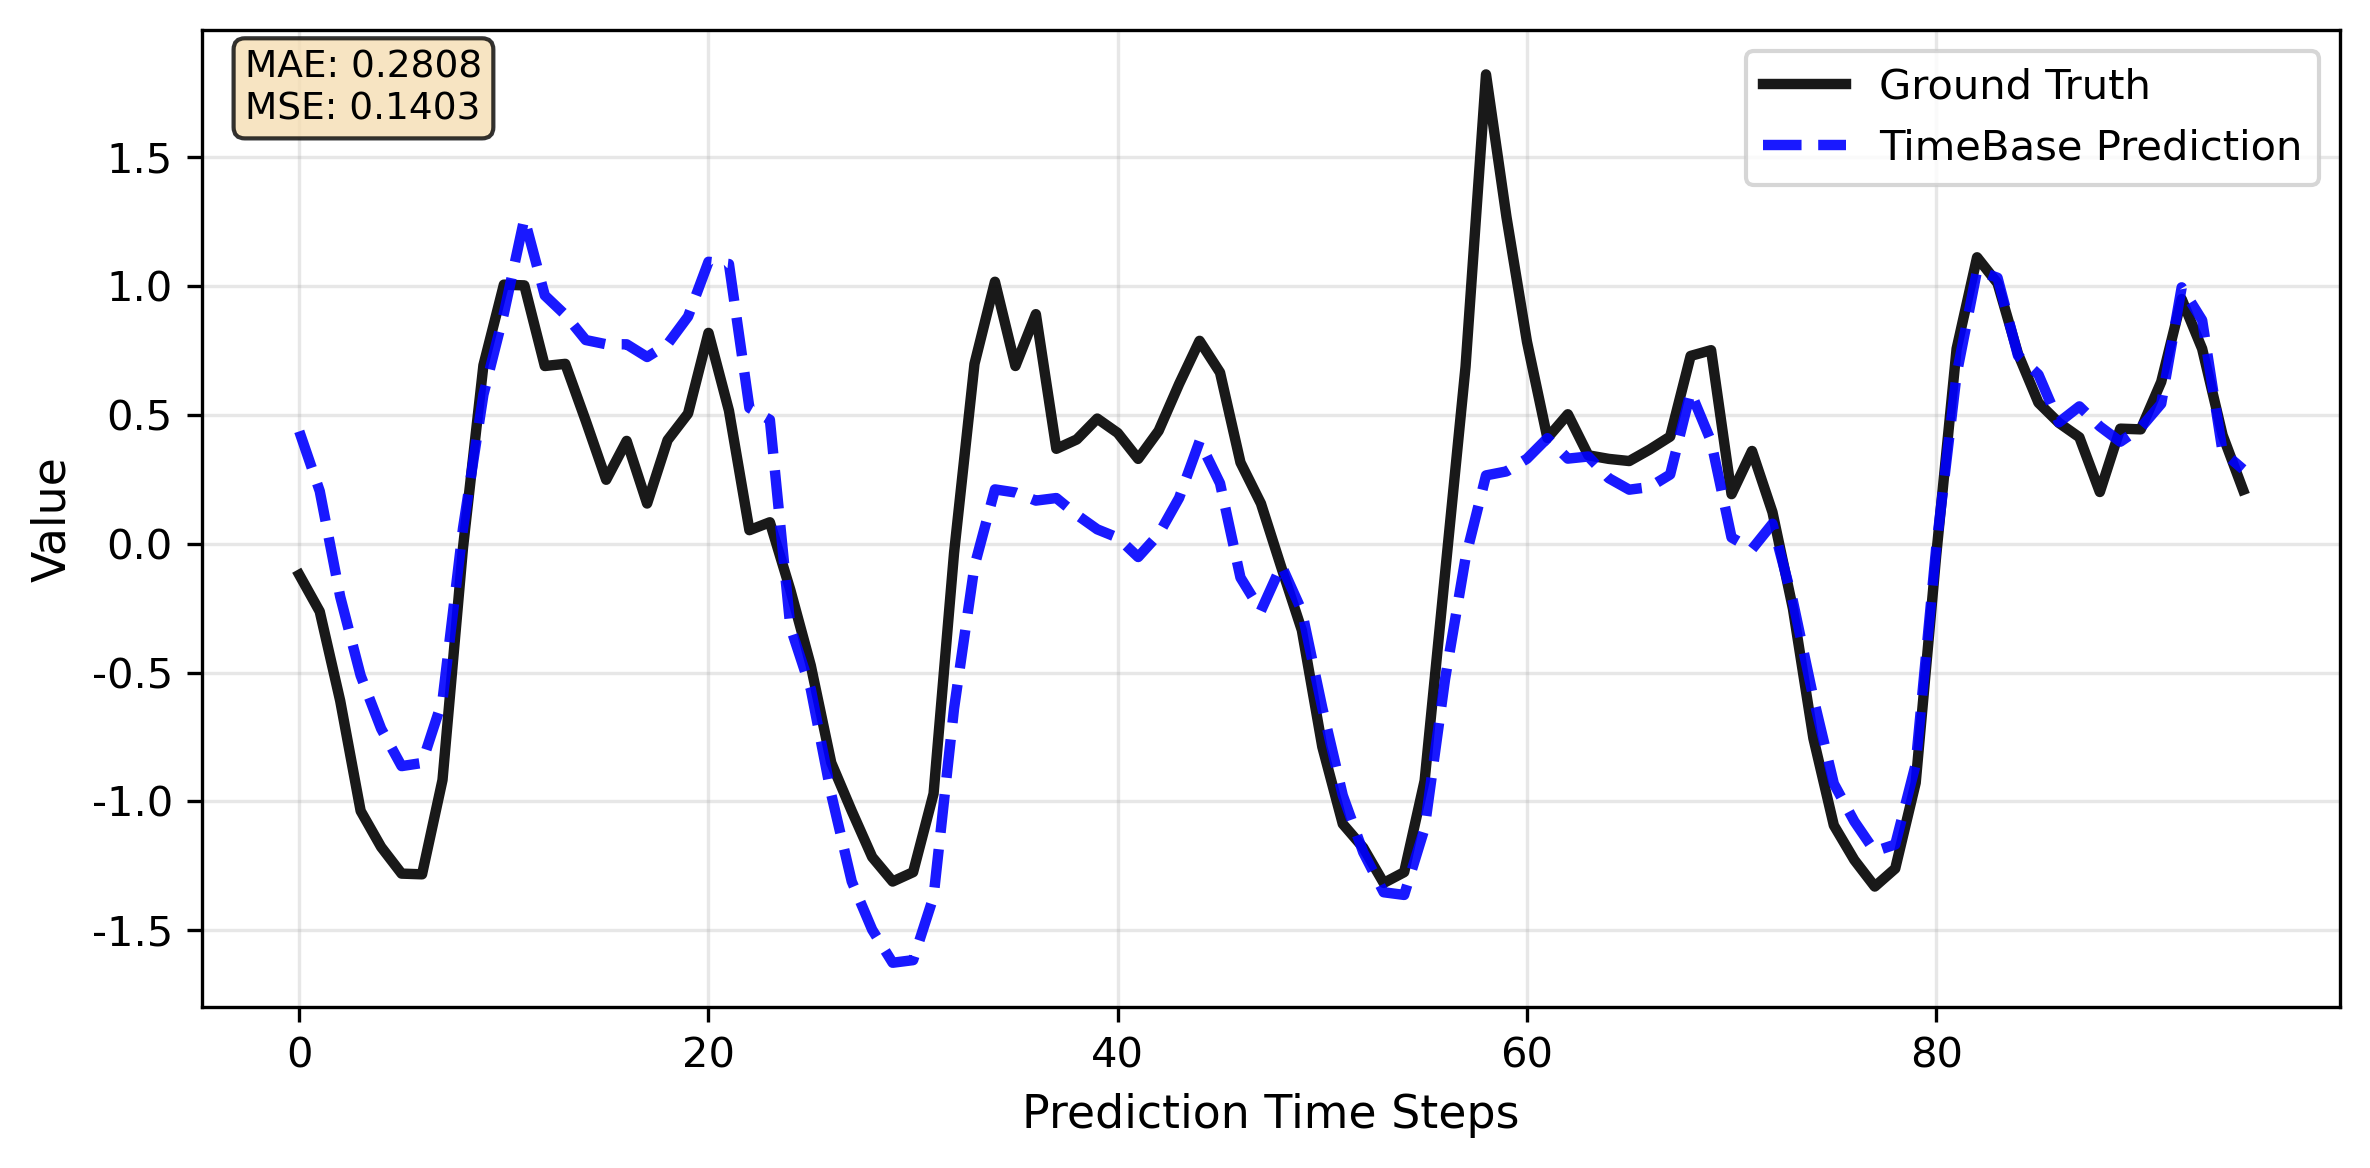
\includegraphics[width=\linewidth]{figures/TimeBase_prediction_20250923_021323.png}
        \caption{TimeBase}
    \end{subfigure}

    \caption{Visualization of forecasting results on Traffic dataset. The black lines stand for the ground truth and the \textcolor{blue}{blue} lines stand for forecasting results.}
\end{figure*}


\subsection{Theoretical Analysis for Phase Tokenization}
\label{sub:theoretical}
\revised{
Under the classical finite-order linear system assumption, the structural dependencies in a time series (especially periodic or quasi-periodic components) are reflected in the rank properties of suitable delay-embedding matrices.

Consider a univariate time series
\[
x_1, x_2, \ldots, x_T.
\]
Fix a collection of delays (lags) \(\tau_1,\ldots,\tau_D\) and a set of reference indices \(s_1,\ldots,s_H\) such that
\(s_h + \tau_D \le T\) for all \(h\).
The corresponding \(D \times H\) delay-embedding matrix is
\[
X =
\begin{bmatrix}
x_{s_1+\tau_1} & x_{s_2+\tau_1} & \cdots & x_{s_H+\tau_1} \\
x_{s_1+\tau_2} & x_{s_2+\tau_2} & \cdots & x_{s_H+\tau_2} \\
\vdots & \vdots &        & \vdots \\
x_{s_1+\tau_D} & x_{s_2+\tau_D} & \cdots & x_{s_H+\tau_D}
\end{bmatrix}.
\]
The classical Hankel matrix is recovered as the special case with unit delay and consecutive indices, e.g.\ \(\tau_d=d-1\) and \(s_h=h\), but our analysis does not rely on this specific structure.

If the series is dominated by periodic or harmonic components, it can often be generated (or well approximated) by a low-dimensional linear dynamical system. In this case, the delay-embedding matrix \(X\) exhibits a natural \textbf{low-rank} structure: its columns lie approximately in a low-dimensional subspace determined by the underlying system dynamics. Only when the series resembles unstructured white noise does the delay-embedding matrix approach full rank.

For a univariate periodic (or quasi-periodic) series, such a delay-embedding admits the factorization
\[
X = A G,
\]
where \(A\) and \(G\) encode, respectively, the delay-dependent responses and the coefficients associated with different reference indices (e.g., days or windows). The parameters \(D\), the choice of delays \(\{\tau_d\}\), and the number of columns \(H\) jointly determine the shape of the embedding.

Thus, we model the data matrix as
\[
X \;=\; A G^\top + N \;\in\;\mathbb{R}^{D\times H},
\]
}
where $A\in\mathbb{R}^{D\times r}$, $G\in\mathbb{R}^{H\times r}$ are column full rank with $\operatorname{rank}(A)=\operatorname{rank}(G)=r$, and $N$ is noise. The true signal is $M = A G^\top$. We assume $r\ll \min(D,H)$.

Patch tokenization corresponds to the row space $\mathrm{Row}(X)$ (the right singular $r$-subspace), while phase tokenization corresponds to the column space $\mathrm{Col}(X)$ (the left singular $r$-subspace).

A shared transformation applies $S\in\mathbb{R}^{H\times H}$ on the hourly dimension:
\[
\blue{X^{\prime}} = X S^\top = A (S G)^\top + \blue{N^{\prime}}.
\]

\revised{
In our formulation, the set $S$ represents a family of linear transformations applied to the input sequence. 
Such transformations frequently arise in practical systems due to sensor delays, timing jitters, or preprocessing procedures including smoothing or temporal alignment.

}

For a matrix $Y$, define the spectral separation as
\[
\mathrm{sep}_r(Y) := \min_{i\le r,\,j>r}|\sigma_i(Y)-\sigma_j(Y)|.
\]
When $\operatorname{rank}(Y)=r$, this equals $\sigma_r(Y)$. In particular,
\[
\delta = \sigma_r(M), \quad \delta'=\sigma_r(MS^\top), \quad
\delta_{\min}=\min(\delta,\delta').
\]
Assume $S$ is invertible on $\mathrm{Col}(G)$, i.e. $\operatorname{rank}(S G)=r$. Define
\[
\kappa := \sigma_{\min}(S|_{\mathrm{Col}(G)})>0.
\]
Moreover, since $\sigma_r(M)\ge\sigma_r(A)\sigma_r(G)$ and 
$\sigma_r(MS^\top)\ge \kappa\sigma_r(A)\sigma_r(G)$, we have the useful bound
\[
\delta_{\min}\;\ge\;\min(1,\kappa)\,\sigma_r(A)\sigma_r(G).
\]

For two $r$-dimensional subspaces $\mathcal U,\mathcal V$, their distance is
\[
d(\mathcal U,\mathcal V) := \|P_{\mathcal U}-P_{\mathcal V}\|_2 \;=\; \sin\Theta_{\max}(\mathcal U,\mathcal V),
\]
where $P_{\mathcal U}$ is the orthogonal projector onto $\mathcal U$. 
This metric satisfies the triangle inequality.

\begin{lemma}[Column space preservation]
Let $M=A G^\top$. If $\operatorname{rank}(S G)=r$, then
\[
\mathrm{Col}(M S^\top) = \mathrm{Col}(M) = \mathrm{Col}(A).
\]
If $\operatorname{rank}(S G)<r$, then the column space shrinks.
\end{lemma}

\begin{lemma}[Row space change]
For $M=A G^\top$,
\[
\mathrm{Row}(M) = \mathrm{Col}(G), \qquad \mathrm{Row}(M S^\top) = \mathrm{Col}(S G).
\]
As a result:
\[
d(\mathrm{Col}(G),\mathrm{Col}(S G))>0 \quad \Longleftrightarrow \quad S(\mathrm{Col}(G)) \neq \mathrm{Col}(G).
\]
\end{lemma}

\begin{lemma}[Wedin’s $\sin\Theta$ theorem]
Let $\widehat M=M+E$ and $\delta=\mathrm{sep}_r(M)>0$. Then
\[
d\big(\mathcal U_r(M),\mathcal U_r(\widehat M)\big) \;\le\; C \frac{\|E\|_2}{\delta},
\]
where $\mathcal U_r(M)$ denotes the leading left singular $r$-subspace of $M$ (the right case is analogous). 
Here $C$ is an absolute constant (often $C\in[2,2\sqrt2]$). The condition $\delta>0$ is necessary.
\end{lemma}

\begin{theorem}
Assume $\operatorname{rank}(S G)=r$ and $\delta,\blue{\delta^{\prime}}>0$. Then:

\begin{enumerate}
\item For phase tokenization,
\[
\begin{aligned}
d\big(\mathcal U_r(X), \mathcal U_r(\blue{X^{\prime}})\big) &\;\le\;
C\Big(\tfrac{\|N\|_2}{\delta}+\tfrac{\|\blue{N^{\prime}}\|_2}{\blue{\delta^{\prime}}}\Big)\\
&\;\le\; C\frac{\|N\|_2+\|\blue{N^{\prime}}\|_2}{\delta_{\min}}.
\end{aligned}
\]
In the noiseless case, Lemma~1 ensures exact invariance, so the distance is $0$.

\item For patch tokenization,
\[
\begin{aligned}
d\big(\mathcal V_r(X), \mathcal V_r(\blue{X^{\prime}})\big) \;\ge\;
d_0 - C\Big(\tfrac{\|N\|_2}{\delta}+\tfrac{\|\blue{N^{\prime}}\|_2}{\blue{\delta^{\prime}}}\Big),
\end{aligned}
\]
where $d_0 := d(\mathrm{Col}(G),\mathrm{Col}(S G))$. If $S(\mathrm{Col}(G))\neq\mathrm{Col}(G)$, then $d_0>0$.
\end{enumerate}
\end{theorem}

\begin{proof}
For phase tokenization, apply the triangle inequality:
\[
\begin{aligned}
&d(\mathcal U_r(X),\mathcal U_r(X'))\\
&\quad\le d(\mathcal U_r(X),\mathcal U_r(M))\\
&\qquad + d(\mathcal U_r(M),\mathcal U_r(MS^\top))\\
&\qquad + d(\mathcal U_r(MS^\top),\mathcal U_r(X')).
\end{aligned}
\]
By Lemma~1 the middle term vanishes, and the two boundary terms are bounded by Wedin’s theorem, yielding the stated inequality.  

For patch tokenization, we have
\[
\begin{aligned}
&d(\mathcal V_r(X),\mathcal V_r(X'))\\
&\quad\ge d(\mathcal V_r(M),\mathcal V_r(MS^\top))\\
&\qquad - d(\mathcal V_r(M),\mathcal V_r(X))\\
&\qquad - d(\mathcal V_r(MS^\top),\mathcal V_r(X')).
\end{aligned}
\]
By Lemma~2 the first term equals $d_0$, and the other two are controlled by Wedin’s theorem, proving the bound.
\end{proof}

In real-world scenarios, slight variations in timing or conditions occur from day to day, so the daily transformations are not exactly identical. 
We model this systematic inconsistency by introducing a small perturbation $\Delta_d$, which captures the mismatch between the ideal linear transformation $S$ and the actual data-generating process.
Suppose each day’s transform is $S_d=S+\Delta_d$ with $\|\Delta_d\|_2\le\varepsilon$. Then
\[
\blue{X^{\prime}} = X S^\top + R, \qquad R_{d,:}=X_{d,:}\Delta_d^\top.
\]
Bounding row by row gives $\|R_{d,:}\|_2 \le \varepsilon\|X_{d,:}\|_2$, hence
\[
\begin{aligned}
\|R\|_F &\le \varepsilon \|X\|_F \quad \Rightarrow \quad \\
\|R\|_2 &\le \varepsilon(\|M\|_F+\|N\|_F).
\end{aligned}
\]

\revised{
The stability of tokenization-induced subspaces measures whether the model is able to maintain consistent internal representations of key periodic or trend components when subjected to these perturbations. 
Correspondingly, the distances between tokenization-induced subspaces provide a quantitative assessment of how much the representation changes, with smaller distances indicating more stable and reliable token features.

Phase-based tokenization exhibits near-invariance under these transformations, offering an inductive bias that is particularly beneficial for real-world forecasting scenarios. 
}

\begin{theorem}[Stability under day-wise perturbations]\label{thm:relaxed}
Under the relaxed model, each day uses $S_d=S+\Delta_d$ with $\|\Delta_d\|_2\le\varepsilon$, so that
\[
X' \;=\; X S^\top + R,\qquad R_{d,:}=X_{d,:}\Delta_d^\top .
\]
Let $X=M+N$ with $M=AG^\top$, $\operatorname{rank}(A)=\operatorname{rank}(G)=r$, and assume
$\operatorname{rank}(SG)=r$ so that $\delta=\sigma_r(M)>0$ and $\delta'=\sigma_r(MS^\top)>0$.
Define $\delta_{\min}=\min(\delta,\delta')$ and $d_0=d(\mathrm{Col}(G),\mathrm{Col}(SG))$.
Then there exists an absolute constant $C\in[2,2\sqrt2]$ such that:
\begin{enumerate}[leftmargin=2em]
\item \textbf{Phase tokenization (left $r$-subspace):}
\[
\begin{aligned}
&d\big(\mathcal U_r(X), \mathcal U_r(X')\big)\\
&\quad\le\;
C\Bigg(
   \frac{\|N\|_2}{\delta}
 + \frac{\|N'\|_2}{\delta'}
 + \frac{\|R\|_2}{\delta'}
\Bigg) \\
&\quad\le\;
C\,\frac{\varepsilon(\|M\|_F+\|N\|_F)
   + \|N\|_2
   + \|N'\|_2}{\delta_{\min}}.
\end{aligned}
\]

\item \textbf{Patch tokenization (right $r$-subspace):}
\[
\begin{aligned}
&d\big(\mathcal V_r(X), \mathcal V_r(X')\big)\\
&\quad\ge\;
d_0 \;-\;
C\Bigg(
   \frac{\|N\|_2}{\delta}
 + \frac{\|N'\|_2}{\delta'}
 + \frac{\|R\|_2}{\delta'}
\Bigg) \\
&\quad\ge\;
d_0 \;-\;
C\,\frac{\varepsilon(\|M\|_F+\|N\|_F)
   + \|N\|_2
   + \|N'\|_2}{\delta_{\min}}.
\end{aligned}
\]
In particular, if $S(\mathrm{Col}(G))=\mathrm{Col}(G)$ then $d_0=0$ and patch tokenization is also preserved up to the same perturbation scale.
\end{enumerate}
Moreover, using $\delta_{\min}\ge \min(1,\kappa)\,\sigma_r(A)\sigma_r(G)$ with
$\kappa=\sigma_{\min}(S|_{\mathrm{Col}(G)})>0$ makes the role of signal strength explicit.
\end{theorem}

\begin{proof}
By row-wise control,
$\|R_{d,:}\|_2\le \varepsilon\|X_{d,:}\|_2$, hence
\[
\begin{aligned}
\|R\|_F&\le \varepsilon\|X\|_F\le \varepsilon(\|M\|_F+\|N\|_F),\\
\|R\|_2&\le \|R\|_F\le \varepsilon(\|M\|_F+\|N\|_F).
\end{aligned}
\]

Insert the chain
\[
\begin{aligned}
X \;\to\; M \;\to\; MS^\top \;\to\; MS^\top+N' \;\to\;{}& X'\\
&=MS^\top+N'+R.
\end{aligned}
\]

For phase subspace $\mathcal U_r$, according to the triangle inequality,
\[
\begin{aligned}
&d\big(\mathcal U_r(X),\mathcal U_r(X')\big)\\
&\quad\le d\big(\mathcal U_r(X),\mathcal U_r(M)\big)\\
&\qquad + d\big(\mathcal U_r(M),\mathcal U_r(MS^\top)\big)\\
&\qquad + d\big(\mathcal U_r(MS^\top),\mathcal U_r(MS^\top+N')\big)\\
&\qquad + d\big(\mathcal U_r(MS^\top+N'),\mathcal U_r(X')\big).
\end{aligned}
\]
The middle term vanishes by Column space preservation (Lemma~1).
Applying Wedin’s $\sin\Theta$ theorem (Lemma~3) to the remaining three perturbations $E\in\{N,\;N',\;R\}$
yields
$C\|N\|_2/\delta + C\|N'\|_2/\delta' + C\|R\|_2/\delta'$.
Use $\delta_{\min}\le\delta,\delta'$ and Step~1 to obtain Item~1.

For patch subspace $\mathcal V_r$, we use the reverse triangle inequality:
\[
\begin{aligned}
&d\big(\mathcal V_r(X),\mathcal V_r(X')\big)\\
&\quad\ge d\big(\mathcal V_r(M),\mathcal V_r(MS^\top)\big)\\
&\qquad - d\big(\mathcal V_r(M),\mathcal V_r(X)\big)\\
&\qquad - d\big(\mathcal V_r(MS^\top),\mathcal V_r(MS^\top+N')\big)\\
&\qquad - d\big(\mathcal V_r(MS^\top+N'),\mathcal V_r(X')\big).
\end{aligned}
\]
The first term equals $d_0$ by Row space change (Lemma~2).
Apply Wedin’s theorem to the other three terms to obtain the final results.
\end{proof}

\revised{
Therefore, we can conclude that our Phase Tokenization performs better than Patch Tokenization when facing periodic perturbations and is more tolerant of mild periodic fluctuations. The above theoretical analysis can be applied to real-world time-series data that have a stable primary period but exhibit small variations.
}



\blue{
\section{Level--Amplitude Coupling on All Splits}
\label{app:coupling_splits}
Table~\ref{tab:coupling} extends Fig.~4(b) of the main manuscript to the training and validation periods. The splits are those of the forecasting experiments: the 12/4/4-month borders on the ETT datasets and 70\%, 10\% and 20\% of the series on the others. The windows span 30 cycles and are shifted by one cycle at a time. For every window, the correlation is taken between the 30 cycle means and the 30 within-cycle RMS deviations. The sign-consistent coupling averages this correlation over the windows of each channel, keeping its sign, and then averages the magnitudes of the channel averages. The shifted-pairing reference computes the same statistic after pairing the cycle means of every window with the RMS deviations of the window half the split later (circularly). The synthetic additive series follows Eq.~(7) of the main manuscript with $\alpha=0$.

\begin{table*}[t]
\centering
\caption{Level--amplitude coupling on every split: sign-consistent coupling, its shifted-pairing reference, and, on the test split, the mean absolute correlation and the share of windows with a positive correlation.}
\label{tab:coupling}
\footnotesize
\setlength{\tabcolsep}{6pt}
\begin{tabular}{lcccccccc}
\toprule
 & \multicolumn{3}{c}{sign-consistent} & \multicolumn{3}{c}{shifted pairing} & \multicolumn{2}{c}{test} \\
\cmidrule(lr){2-4}\cmidrule(lr){5-7}\cmidrule(lr){8-9}
Dataset & train & val & test & train & val & test & mean $|\mathrm{corr}|$ & positive \\
\midrule
Synthetic additive series & 0.00 & 0.05 & 0.02 & 0.00 & 0.03 & 0.01 & 0.14 & 0.47 \\
\midrule
ETTm2 & 0.10 & 0.10 & 0.10 & 0.06 & 0.05 & 0.07 & 0.26 & 0.52 \\
ETTh2 & 0.17 & 0.19 & 0.12 & 0.04 & 0.08 & 0.07 & 0.27 & 0.57 \\
ETTm1 & 0.20 & 0.39 & 0.38 & 0.10 & 0.13 & 0.10 & 0.46 & 0.49 \\
Weather & 0.37 & 0.36 & 0.41 & 0.09 & 0.11 & 0.12 & 0.45 & 0.68 \\
ETTh1 & 0.28 & 0.32 & 0.45 & 0.05 & 0.12 & 0.13 & 0.49 & 0.60 \\
Electricity & 0.54 & 0.55 & 0.50 & 0.07 & 0.11 & 0.12 & 0.55 & 0.84 \\
Traffic & 0.86 & 0.86 & 0.89 & 0.29 & 0.25 & 0.27 & 0.89 & 1.00 \\
\bottomrule
\end{tabular}
\end{table*}
}

\bibliographystyle{spmpsci}
\bibliography{references}

\end{document}
